\chapter{Mass resolution}
\label{app:Massresolution}
Figure \ref{fig:massresolution_all} shows the fits to all bins of \Dz\proton mass for the determination of the mass resolution.
The whole method and prodecure is described in section \ref{sec:Massresolution}.
\begin{figure}[tb]
    \centering
	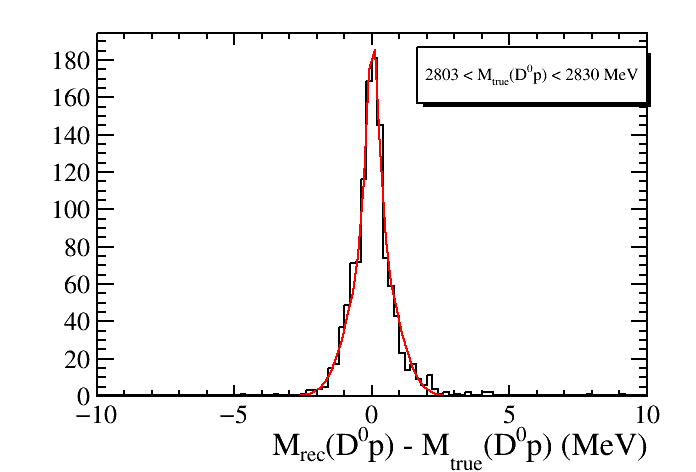
\includegraphics[width=0.32\textwidth]{LbToD0p/massresolution/massresolution_00}
	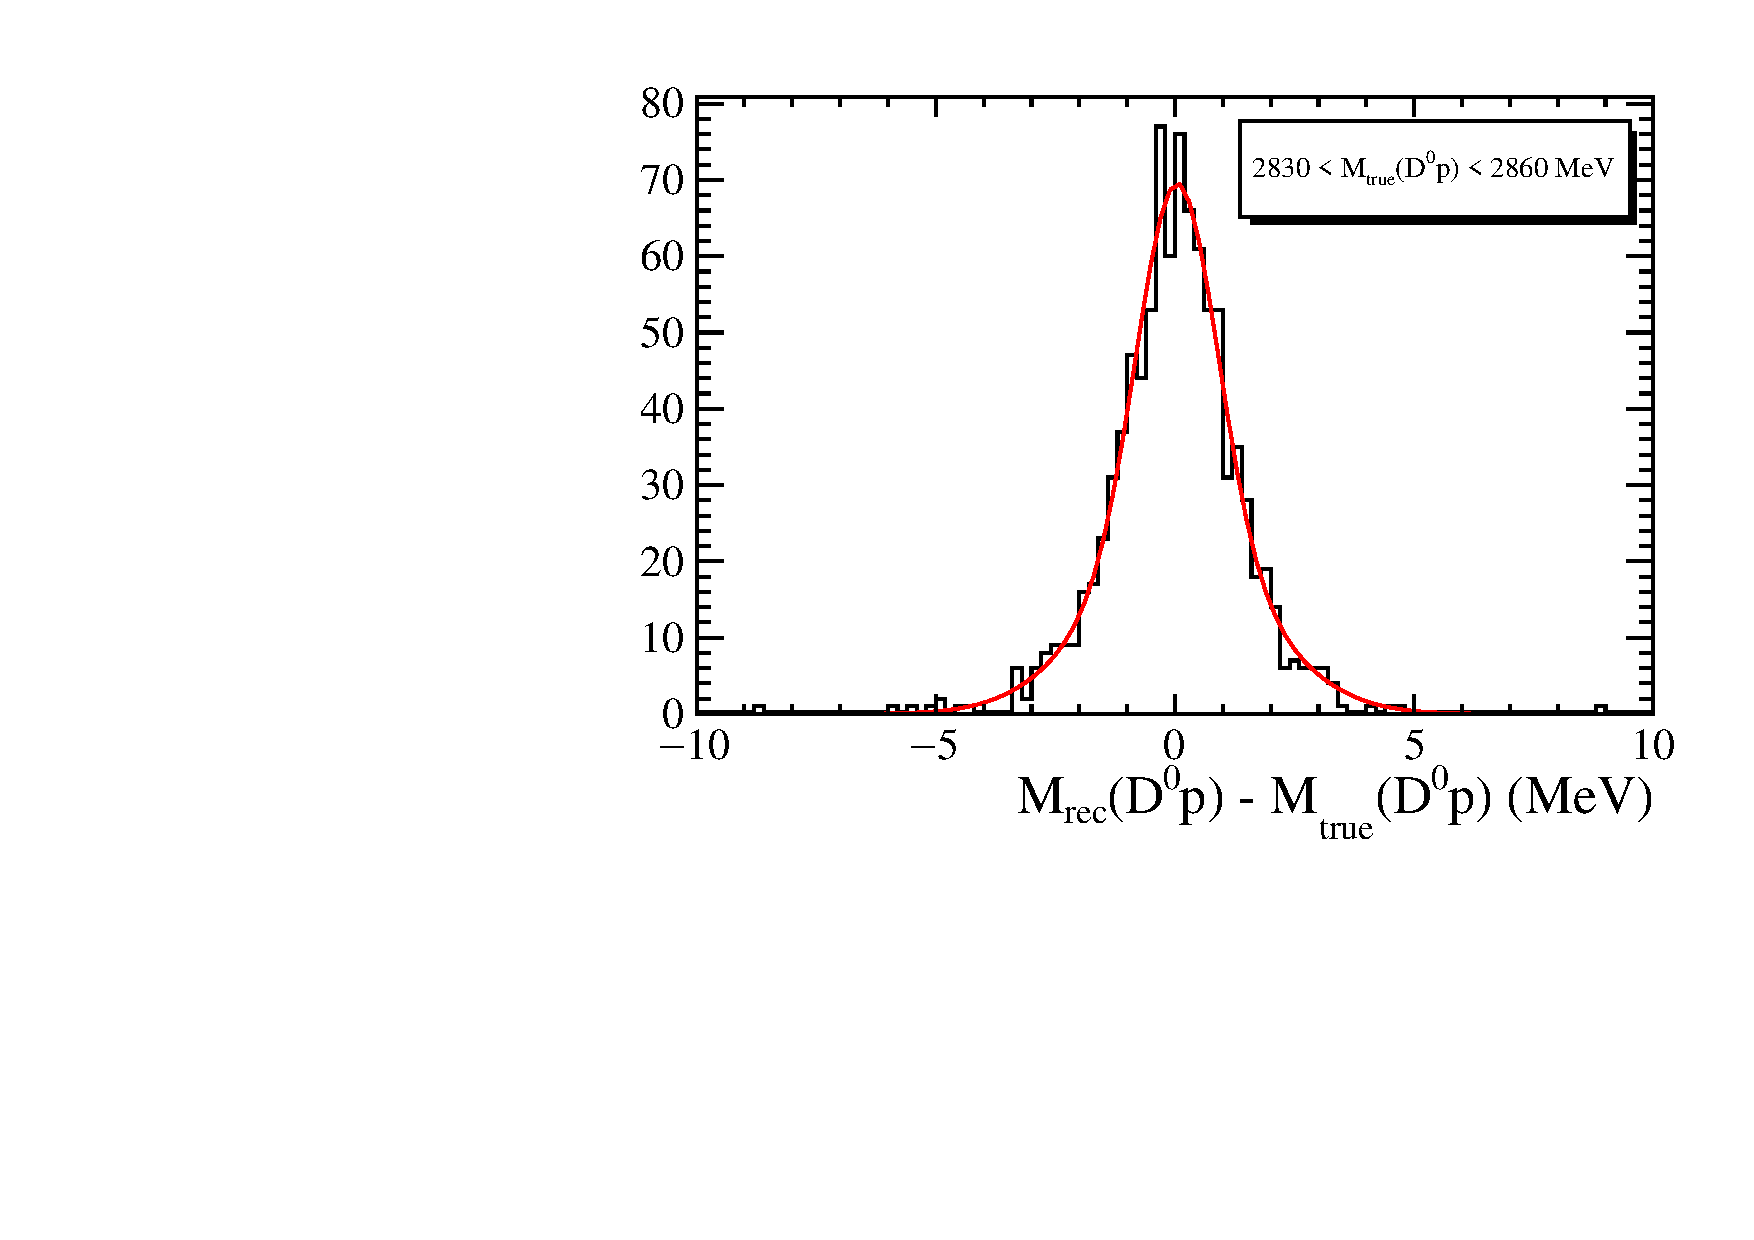
\includegraphics[width=0.32\textwidth]{LbToD0p/massresolution/massresolution_01}
	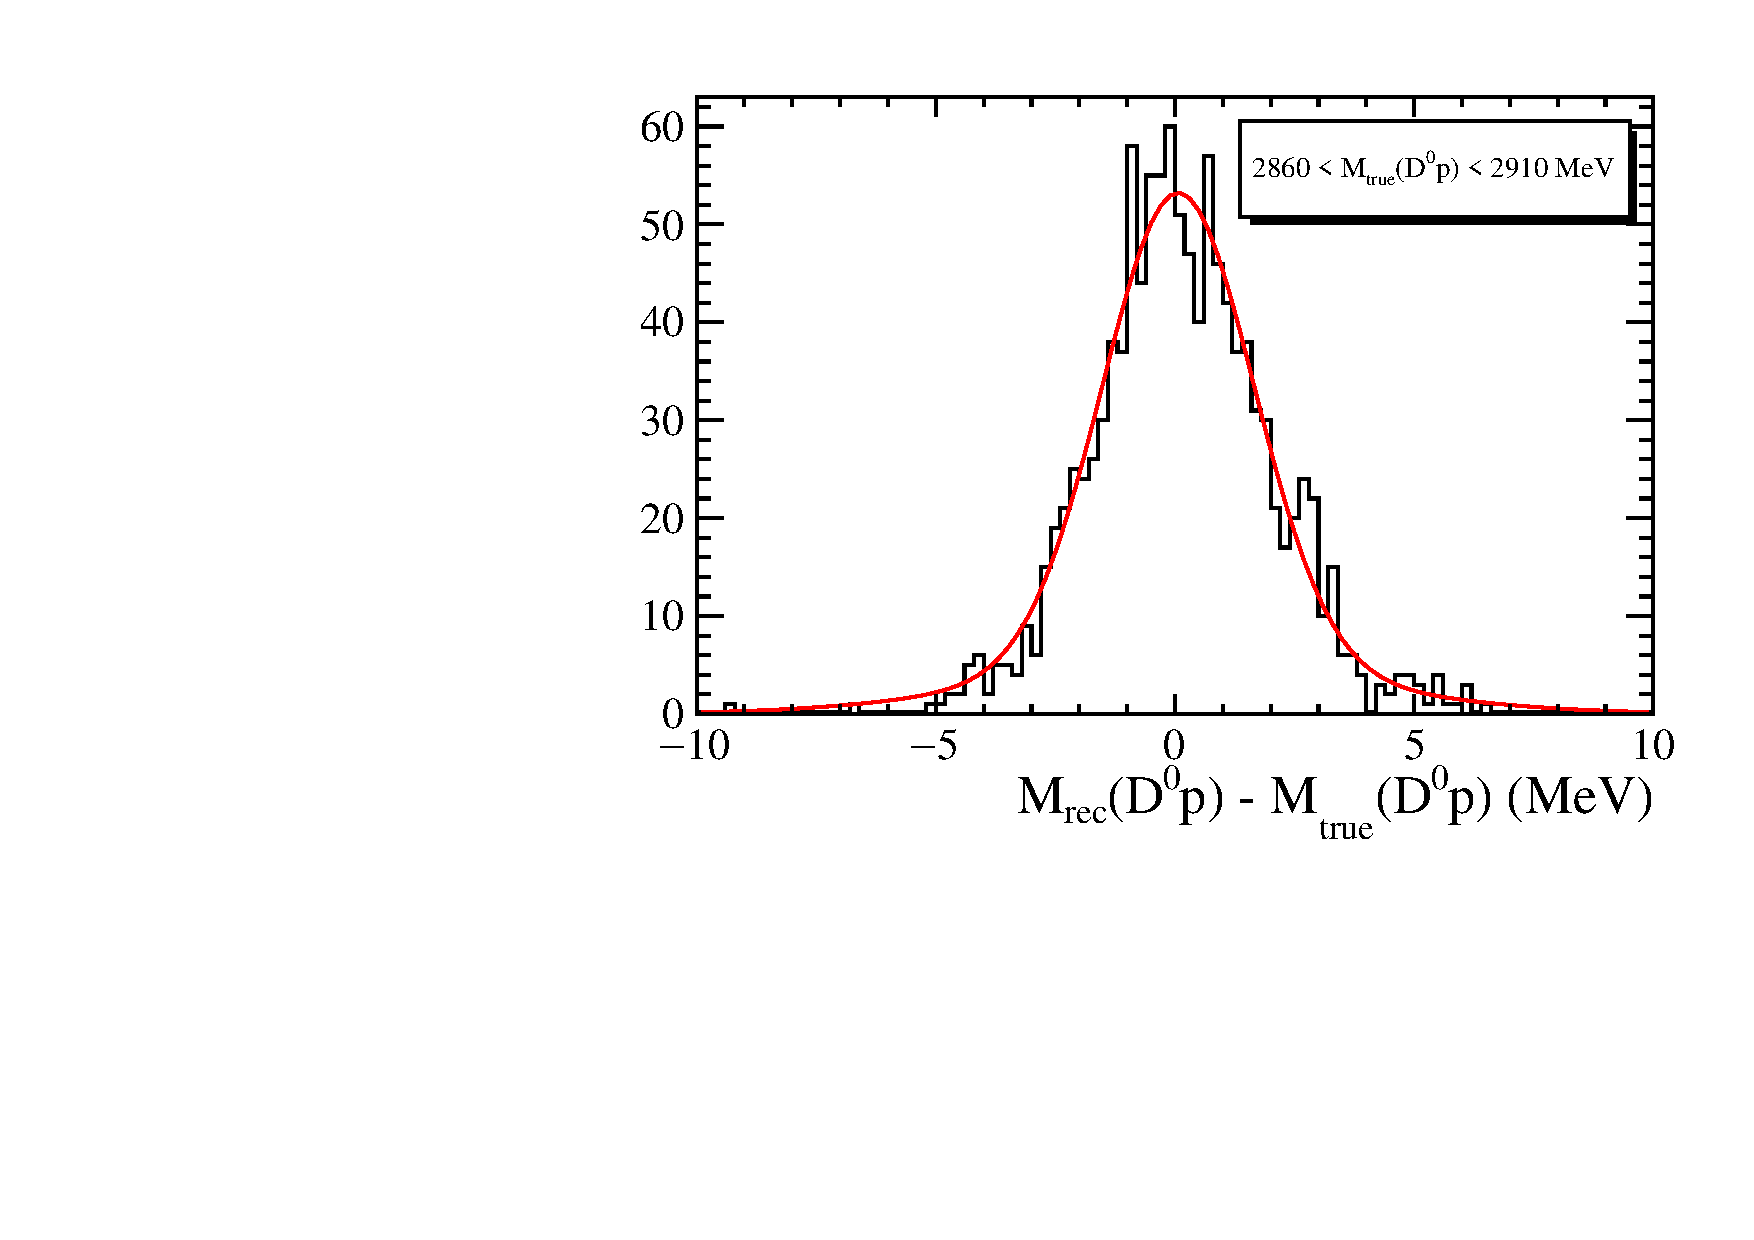
\includegraphics[width=0.32\textwidth]{LbToD0p/massresolution/massresolution_02} \\
	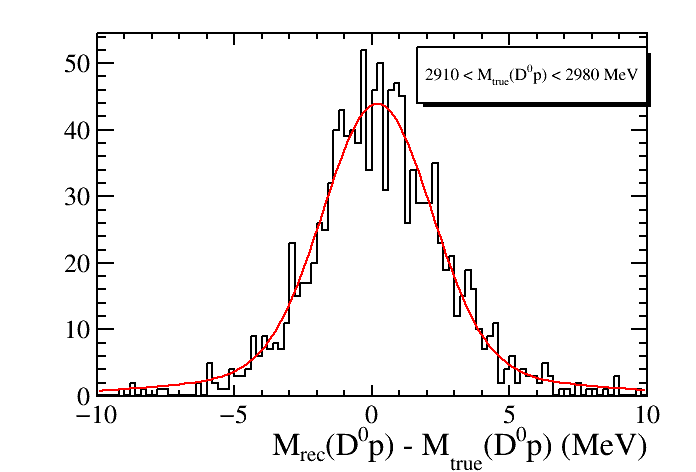
\includegraphics[width=0.32\textwidth]{LbToD0p/massresolution/massresolution_03}
	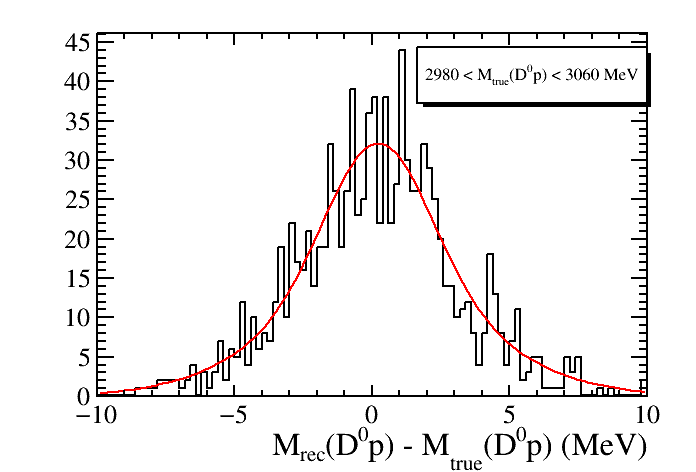
\includegraphics[width=0.32\textwidth]{LbToD0p/massresolution/massresolution_04}
	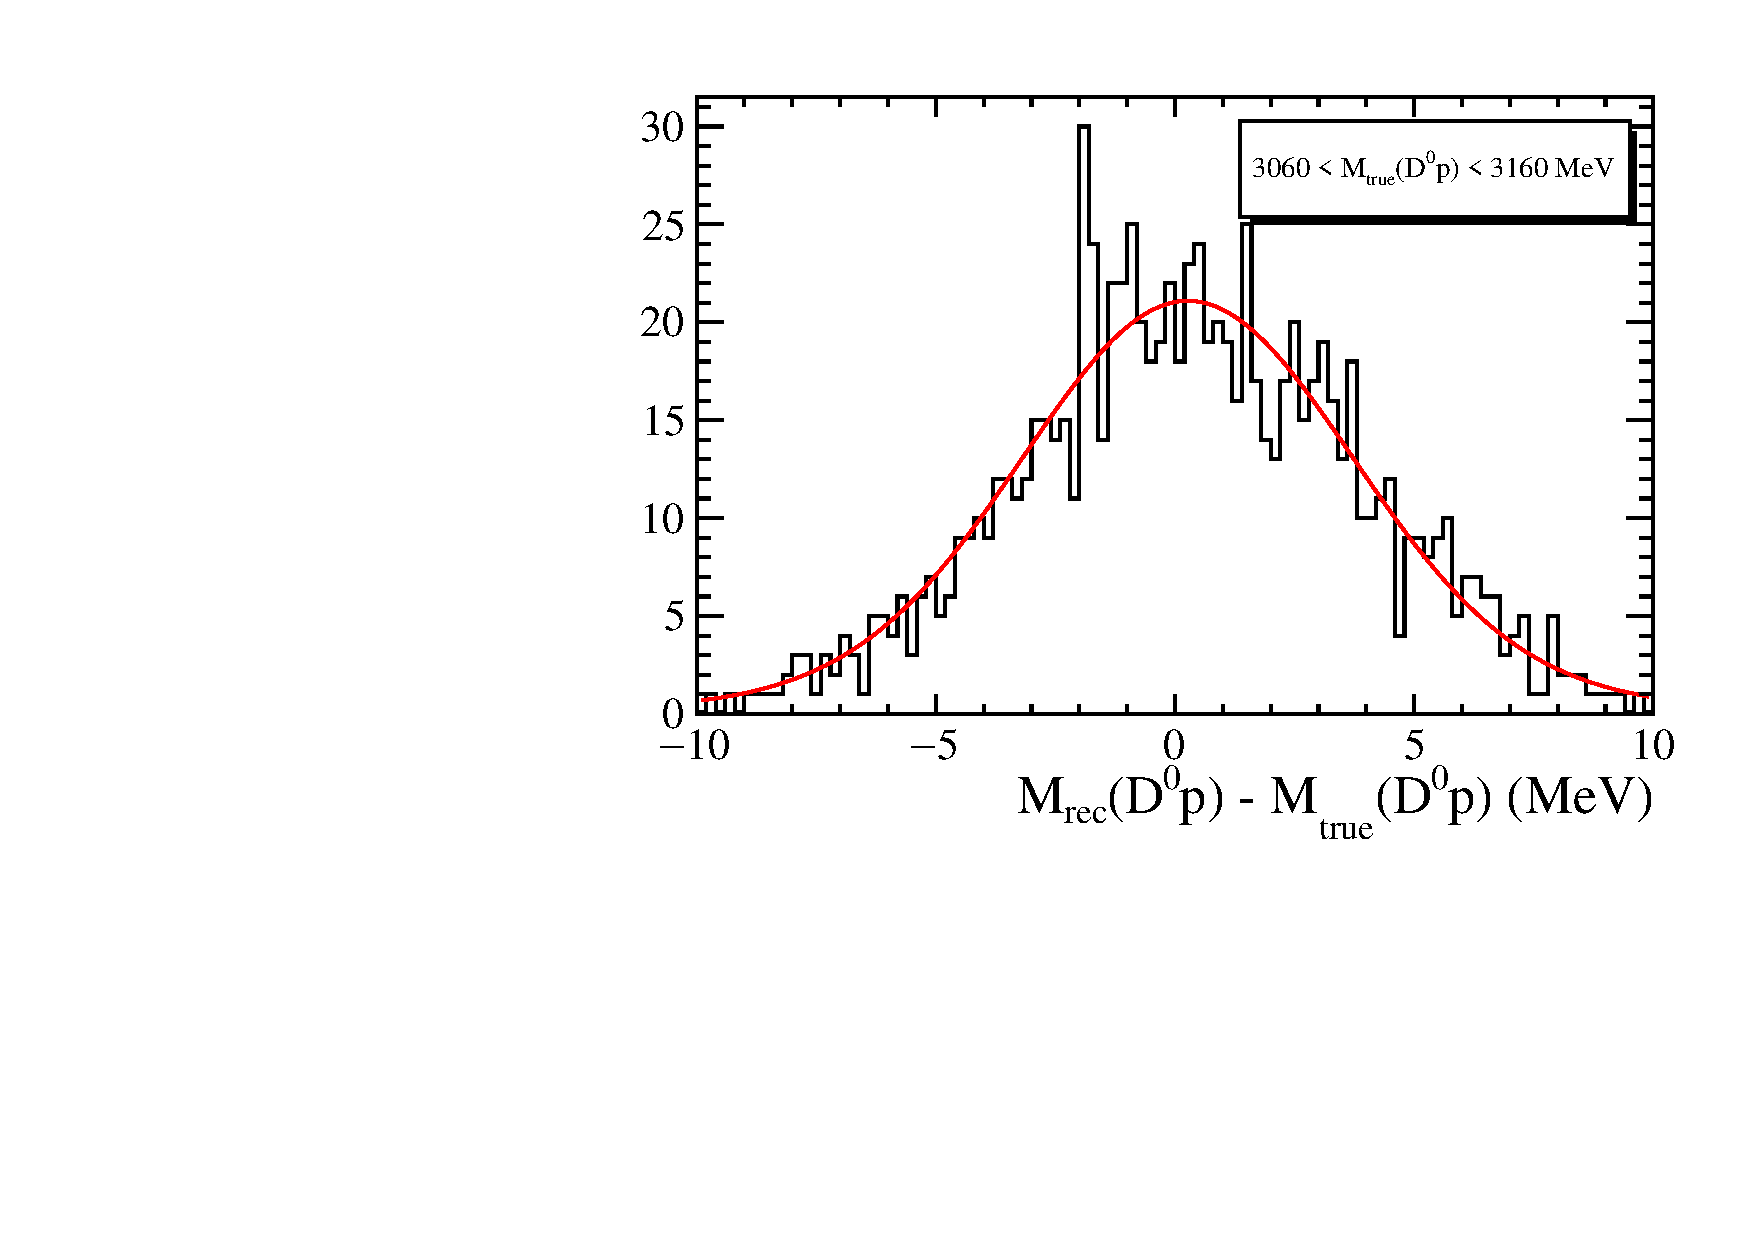
\includegraphics[width=0.32\textwidth]{LbToD0p/massresolution/massresolution_05} \\
	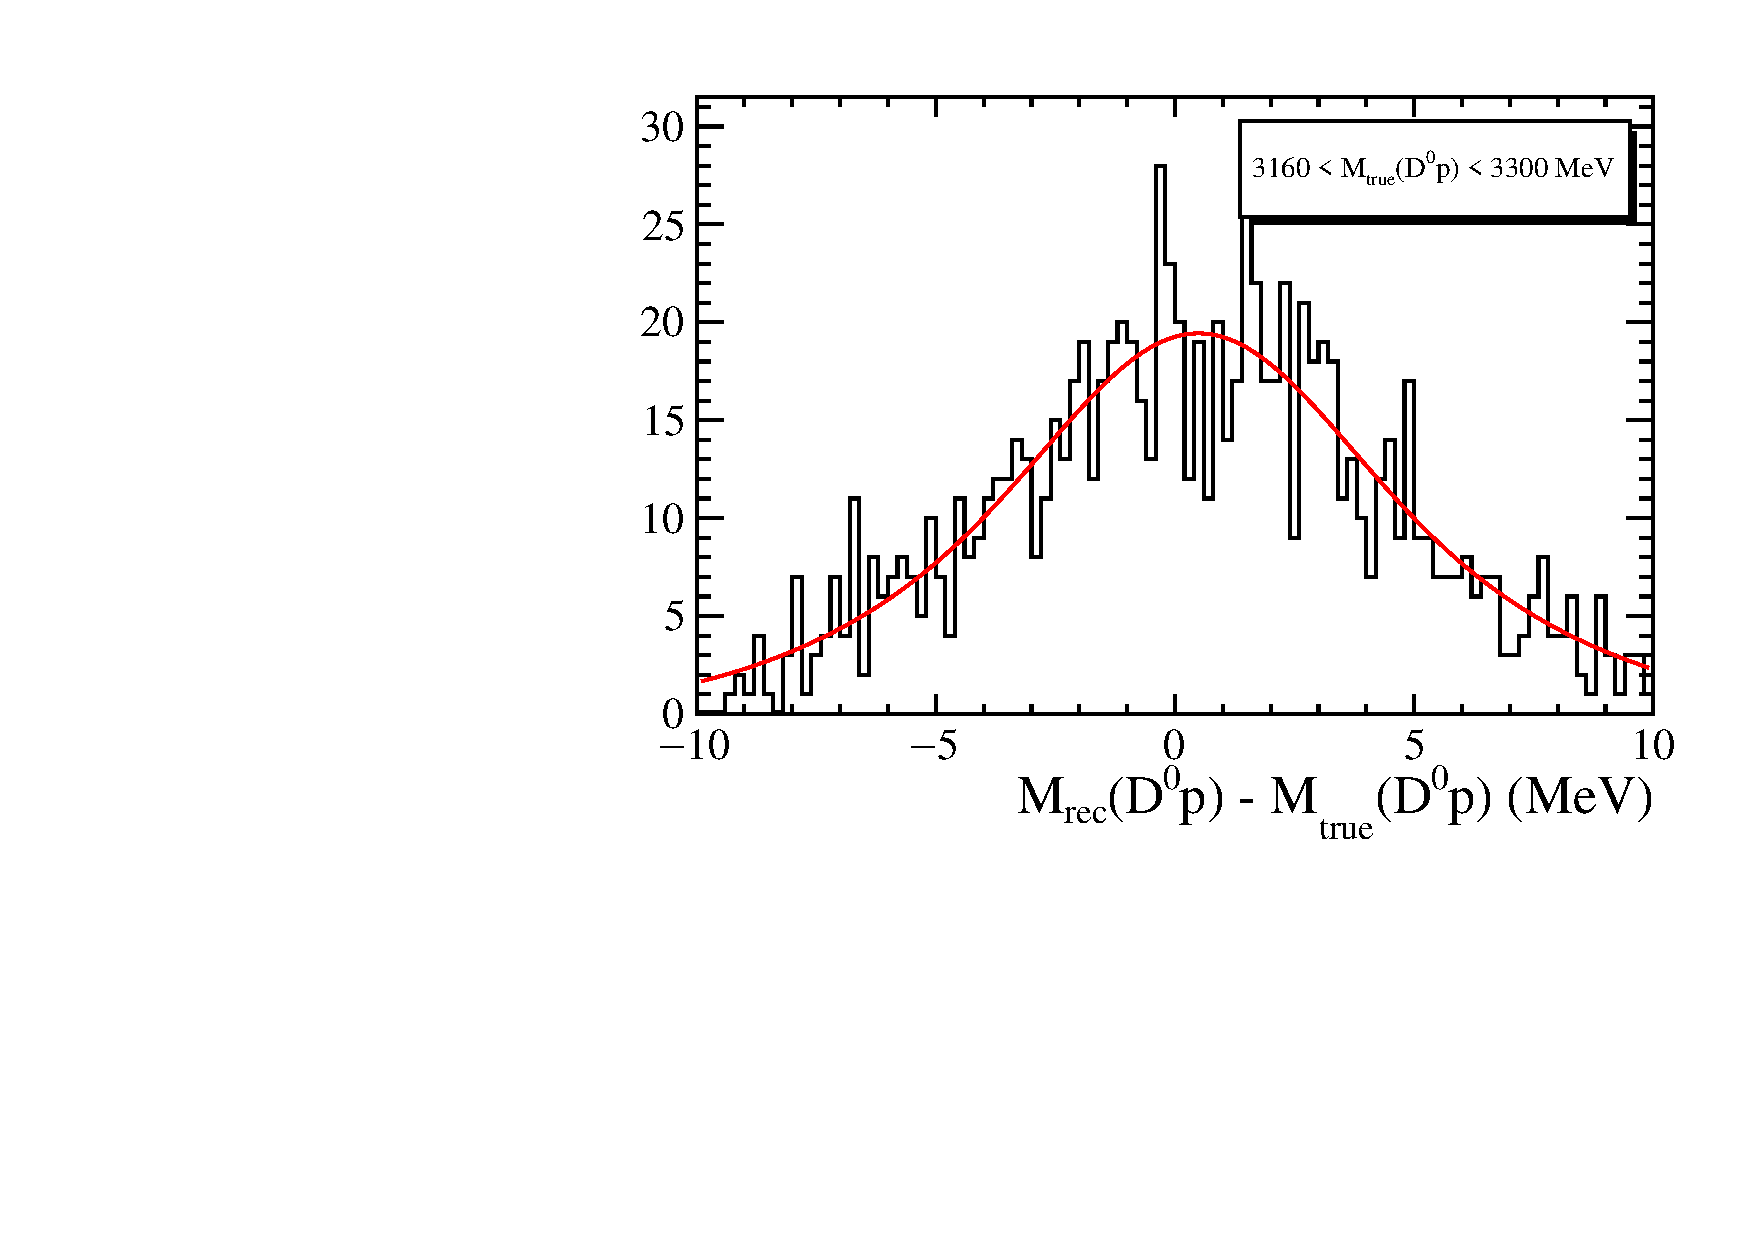
\includegraphics[width=0.32\textwidth]{LbToD0p/massresolution/massresolution_06}
	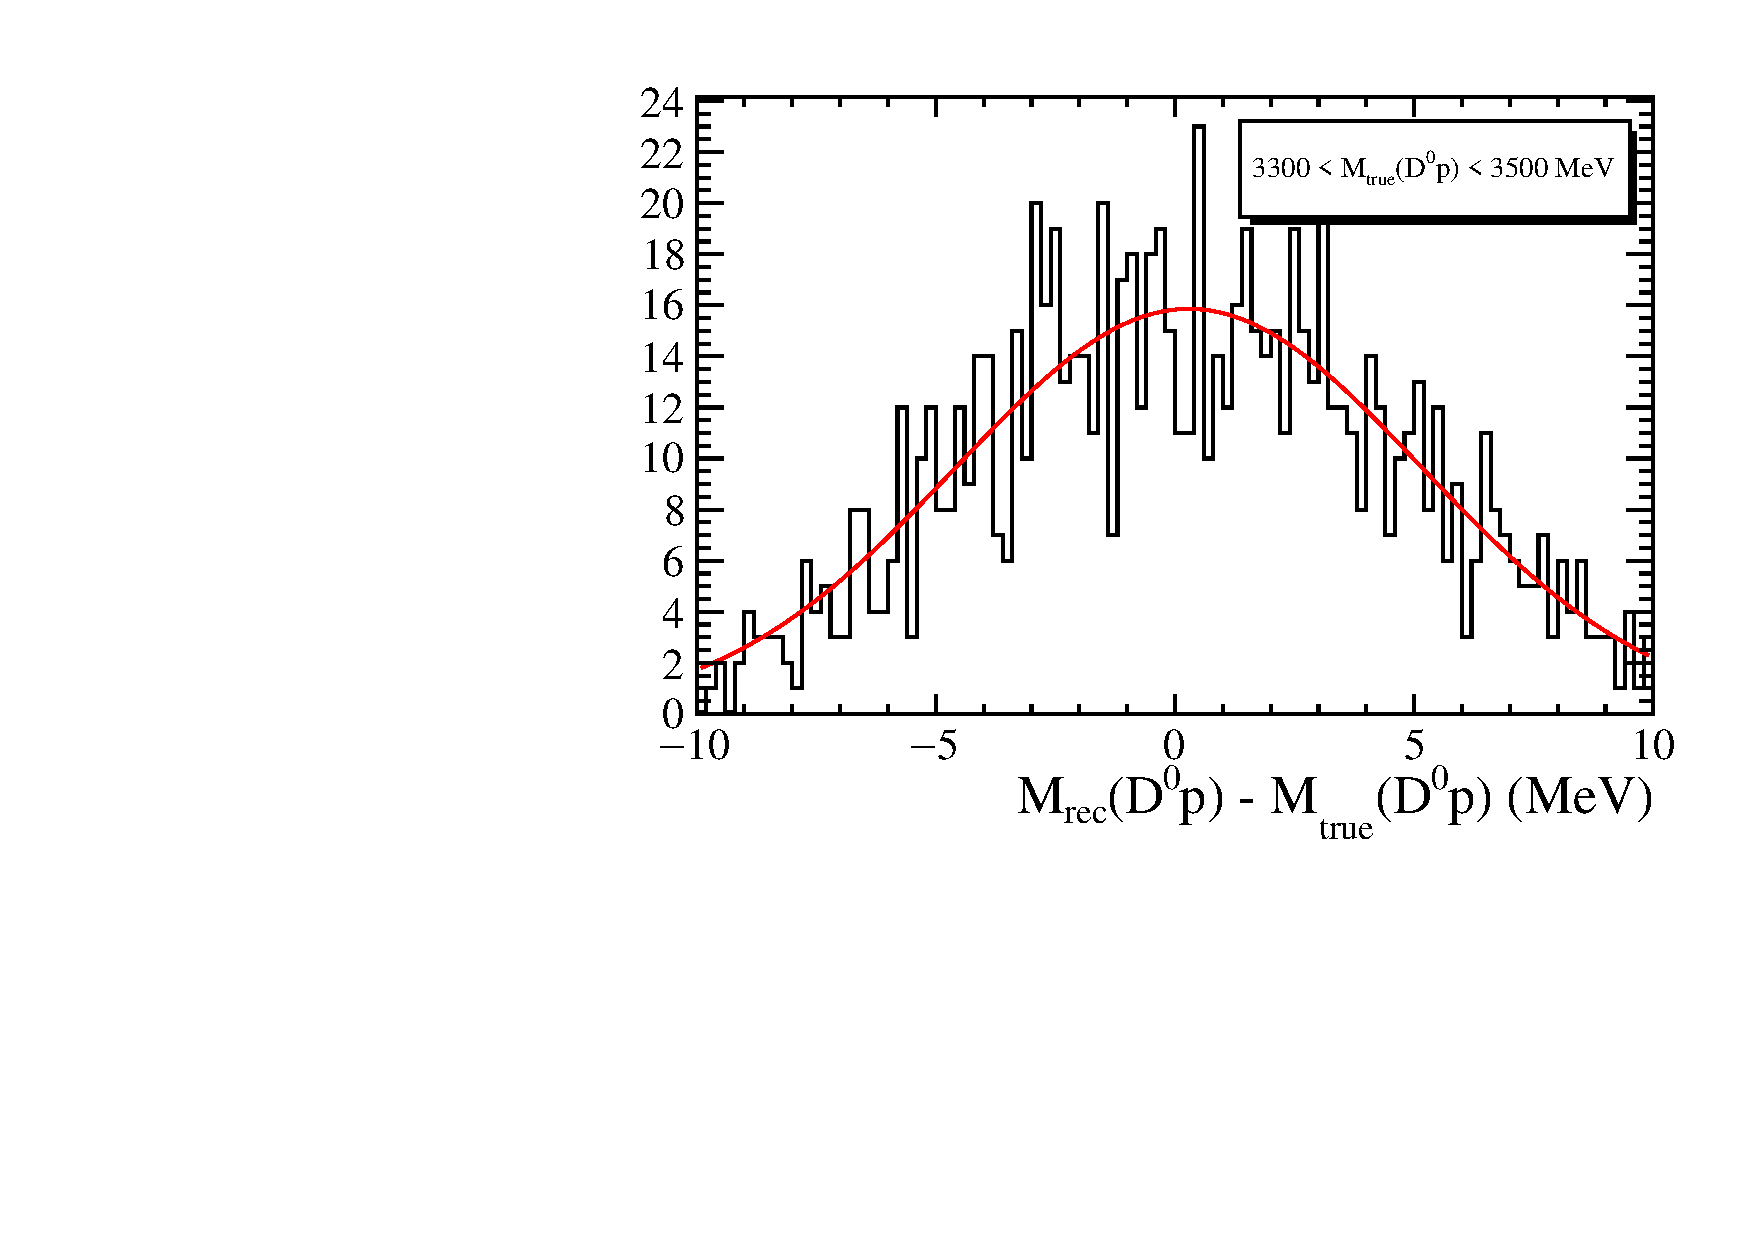
\includegraphics[width=0.32\textwidth]{LbToD0p/massresolution/massresolution_07}
	\caption{Fit of a double Gaussian to the difference between generated and reconstructed \Dz\proton mass (simulation sample) in different bins of true \Dz\proton). The width of distributions corresponds to the mass resolution for the respective bin.}
    \label{fig:massresolution_all}
\end{figure}

\chapter{Reweighting of \LbToDpmunuX decay simulation}
\label{app:Reweight_D0p}
Figure \ref{fig:reweight_D0p_app} shows several more comparisons of data and simulation before and after reweighting.
More on the reweighting process can be found in section \ref{sec:Reweight_D0p}.
\begin{figure}[tb]
    \centering
	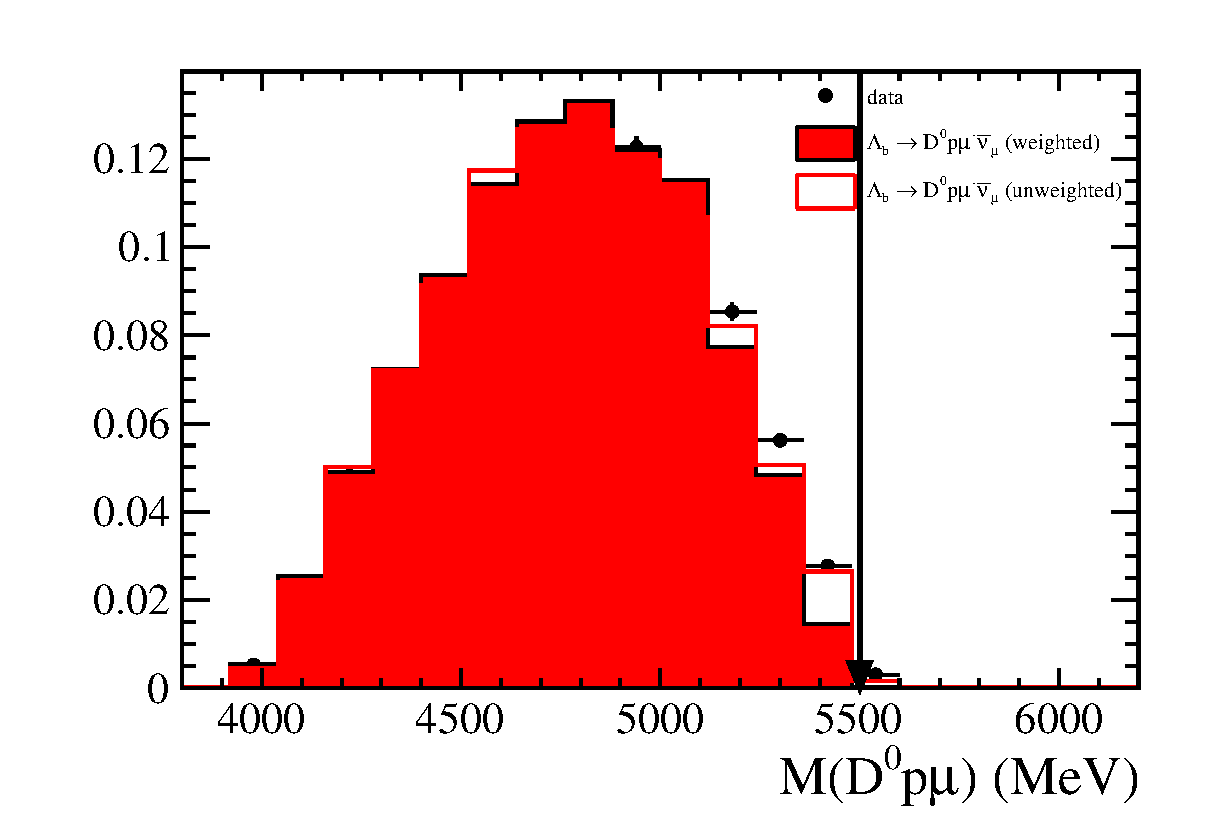
\includegraphics[width=0.32\textwidth]{LbToD0p/comparisons/3D/mD0p_mD0mu_mD0pmu/20Bins/20.0MaxWeight/Bh_M}
	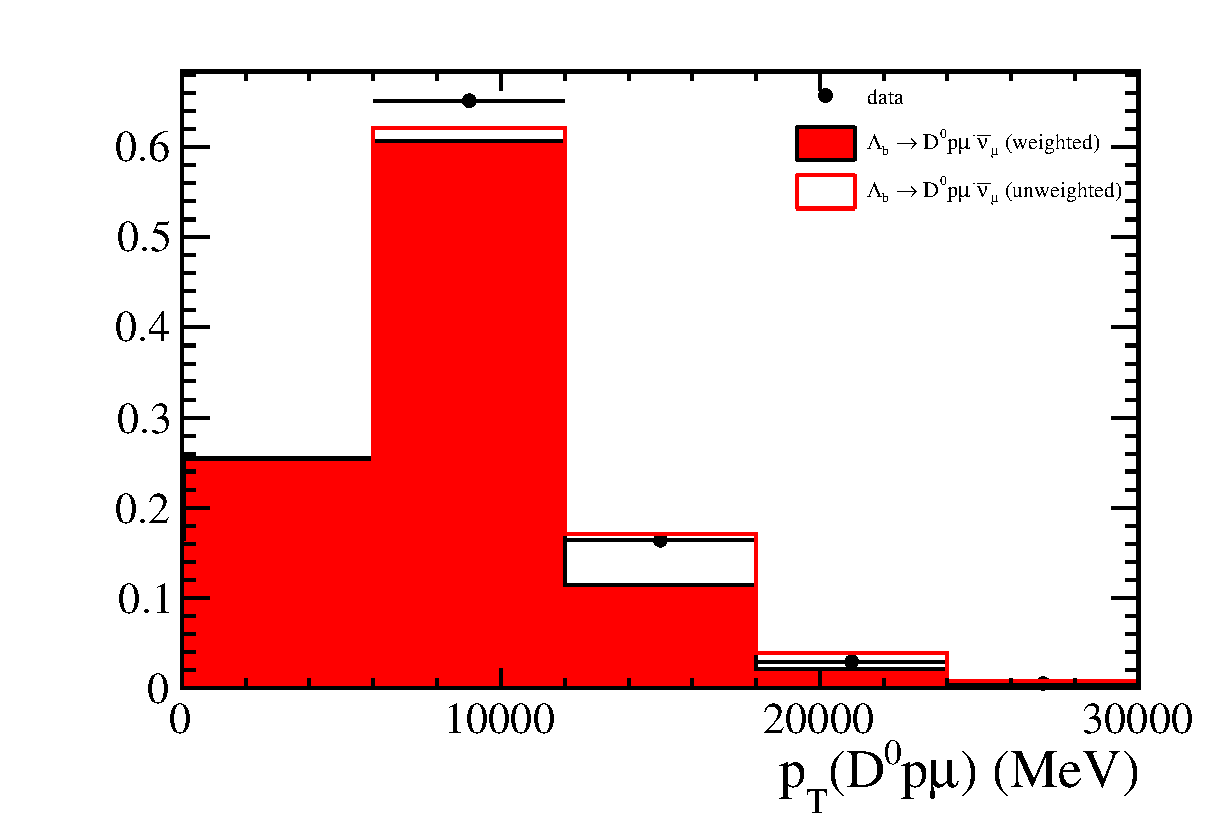
\includegraphics[width=0.32\textwidth]{LbToD0p/comparisons/3D/mD0p_mD0mu_mD0pmu/20Bins/20.0MaxWeight/Bh_PT}
	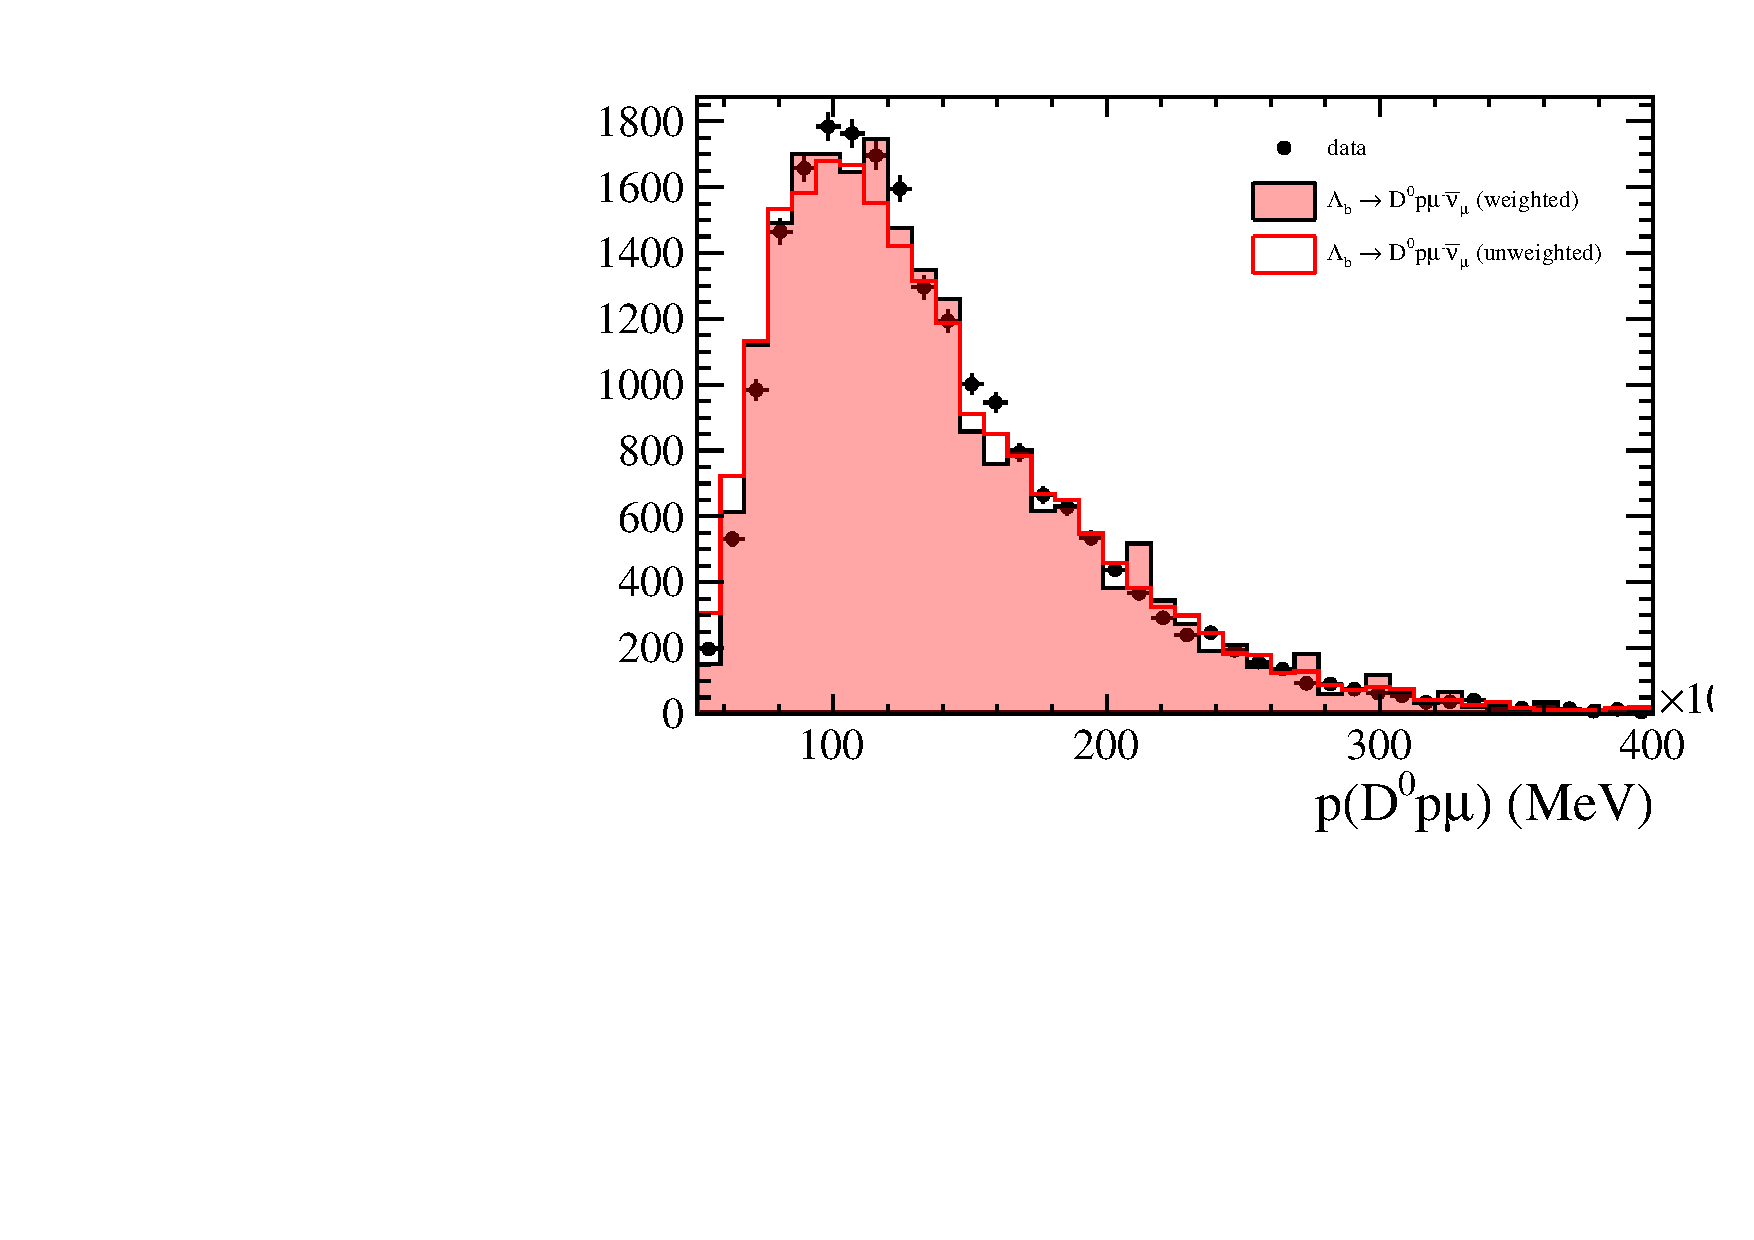
\includegraphics[width=0.32\textwidth]{LbToD0p/comparisons/3D/mD0p_mD0mu_mD0pmu/20Bins/20.0MaxWeight/Bh_P}          \\
	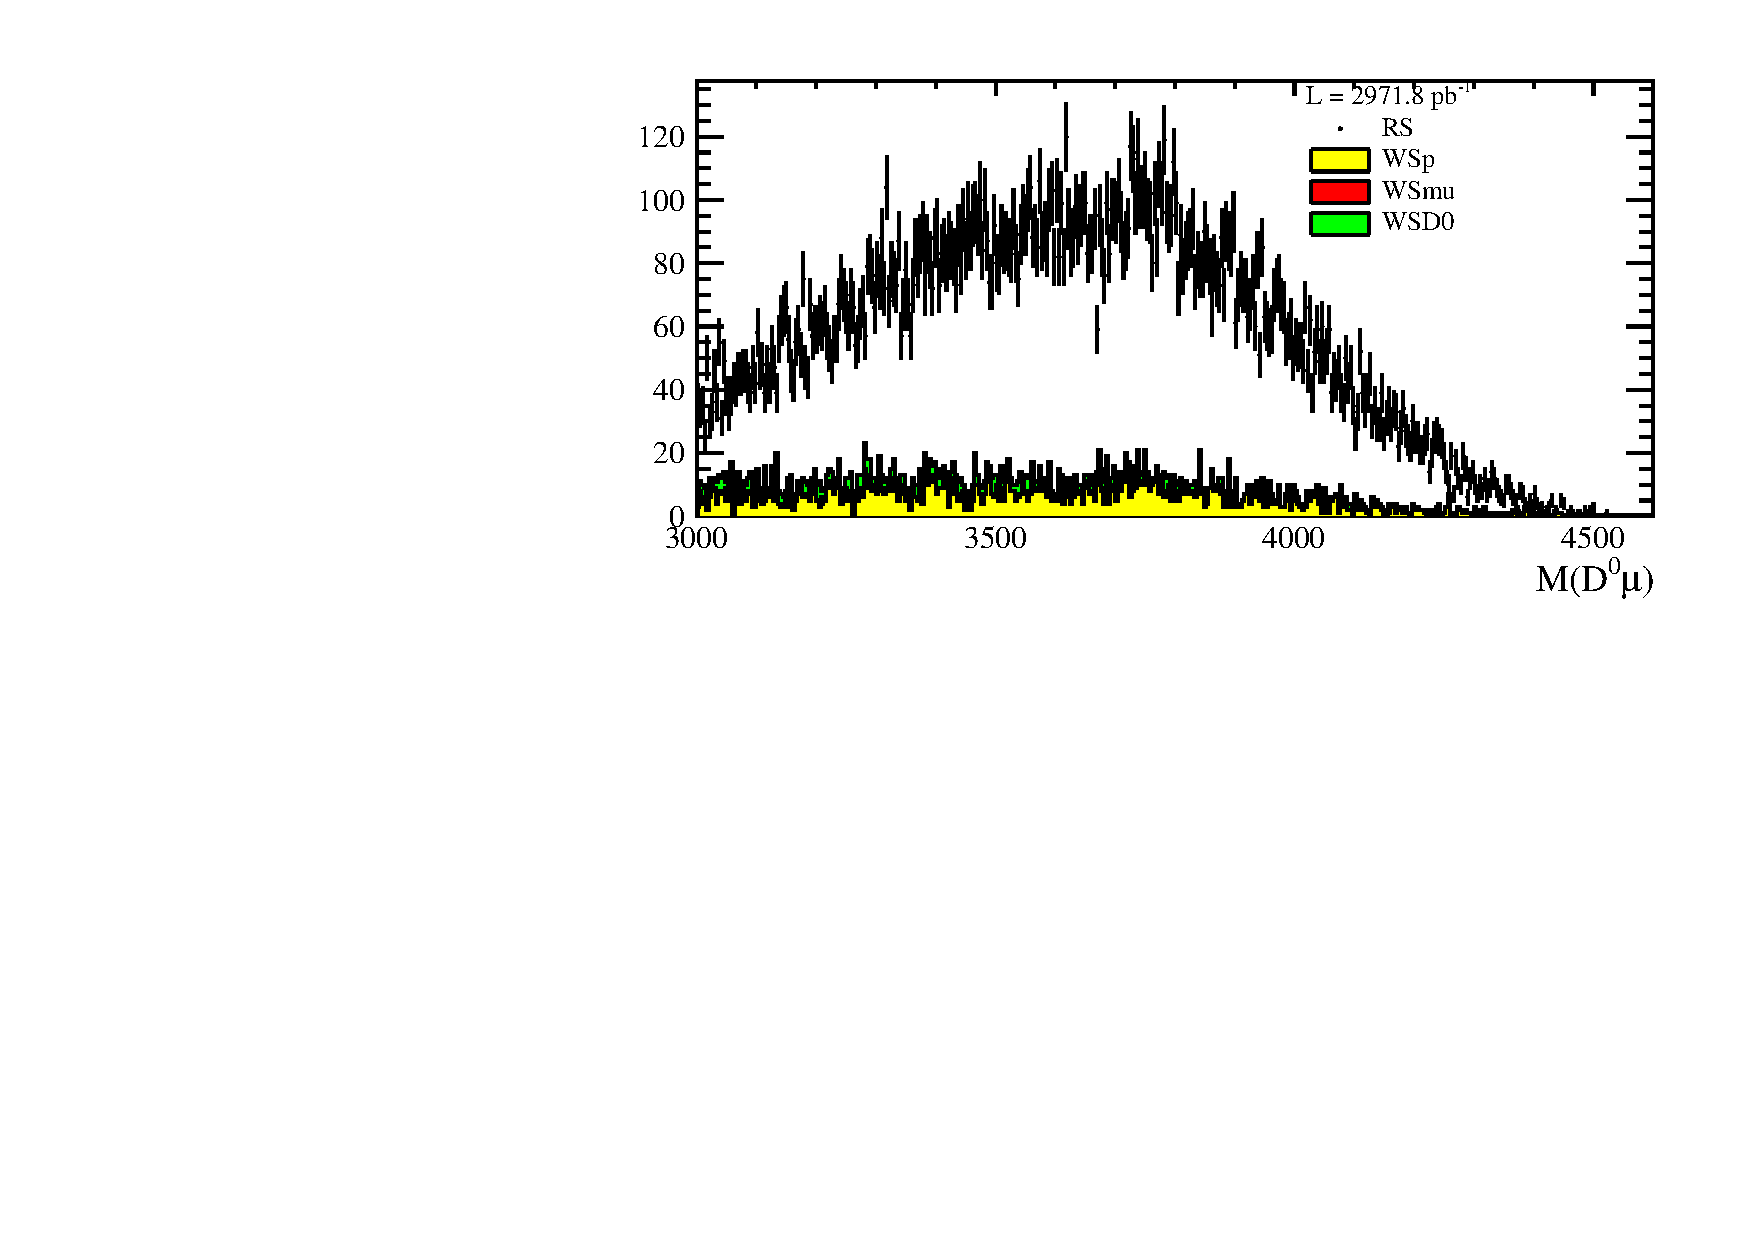
\includegraphics[width=0.32\textwidth]{LbToD0p/comparisons/3D/mD0p_mD0mu_mD0pmu/20Bins/20.0MaxWeight/B_M}           
	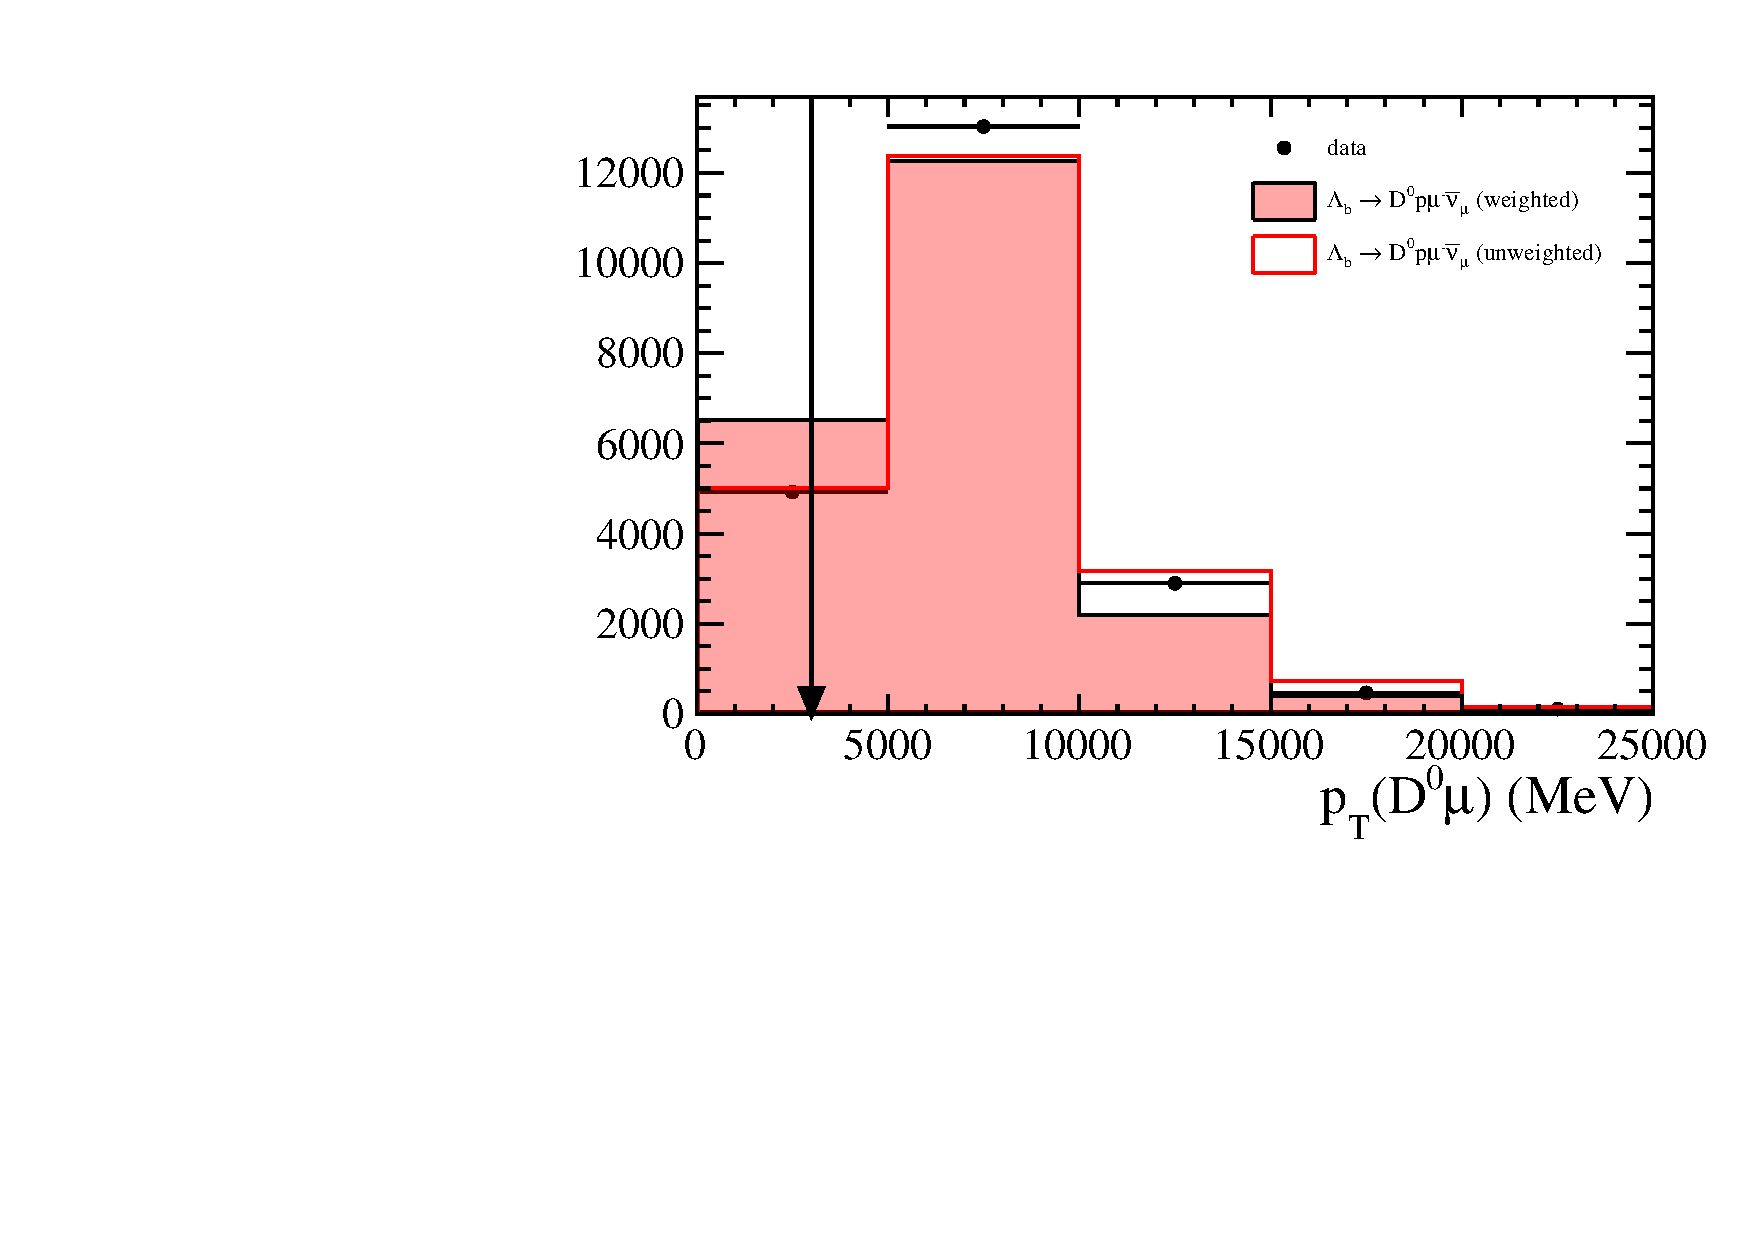
\includegraphics[width=0.32\textwidth]{LbToD0p/comparisons/3D/mD0p_mD0mu_mD0pmu/20Bins/20.0MaxWeight/B_PT}
	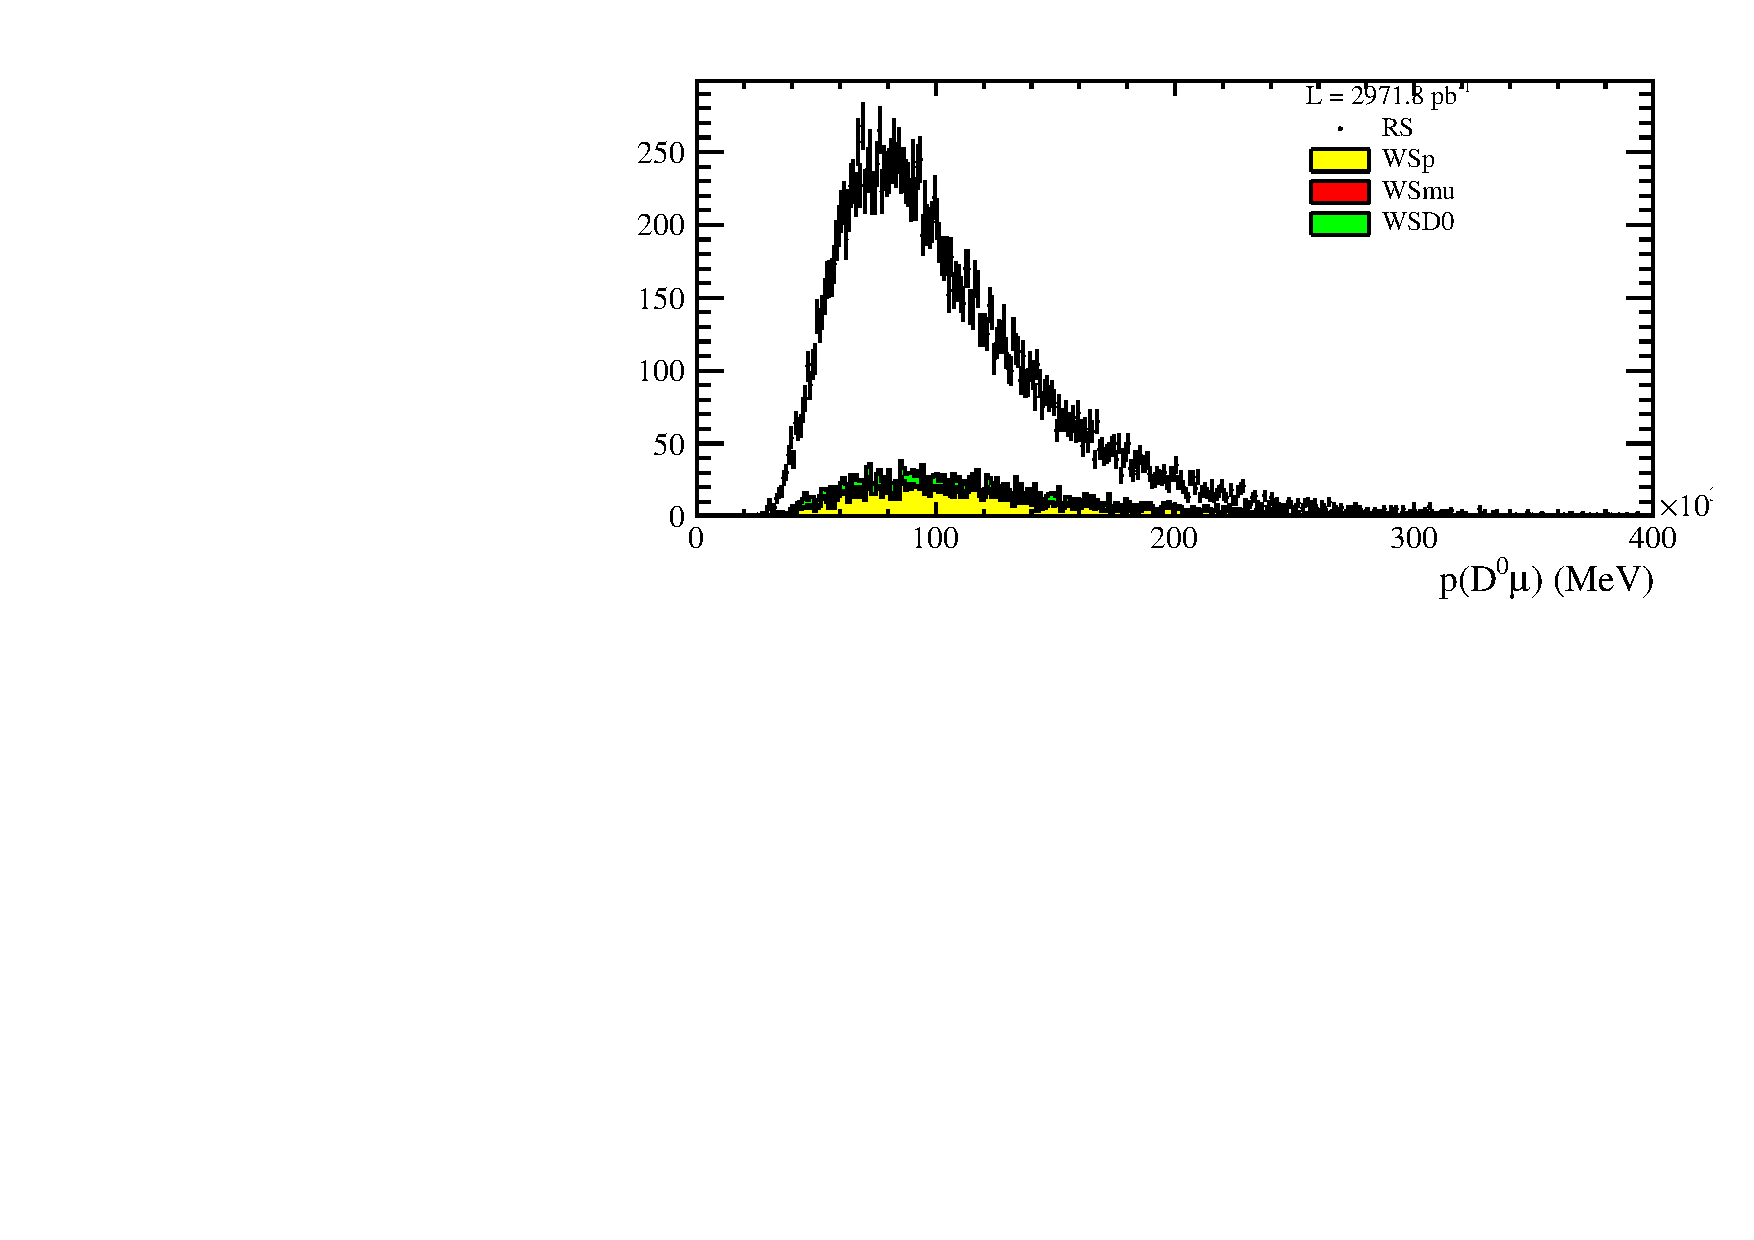
\includegraphics[width=0.32\textwidth]{LbToD0p/comparisons/3D/mD0p_mD0mu_mD0pmu/20Bins/20.0MaxWeight/B_P}           \\
    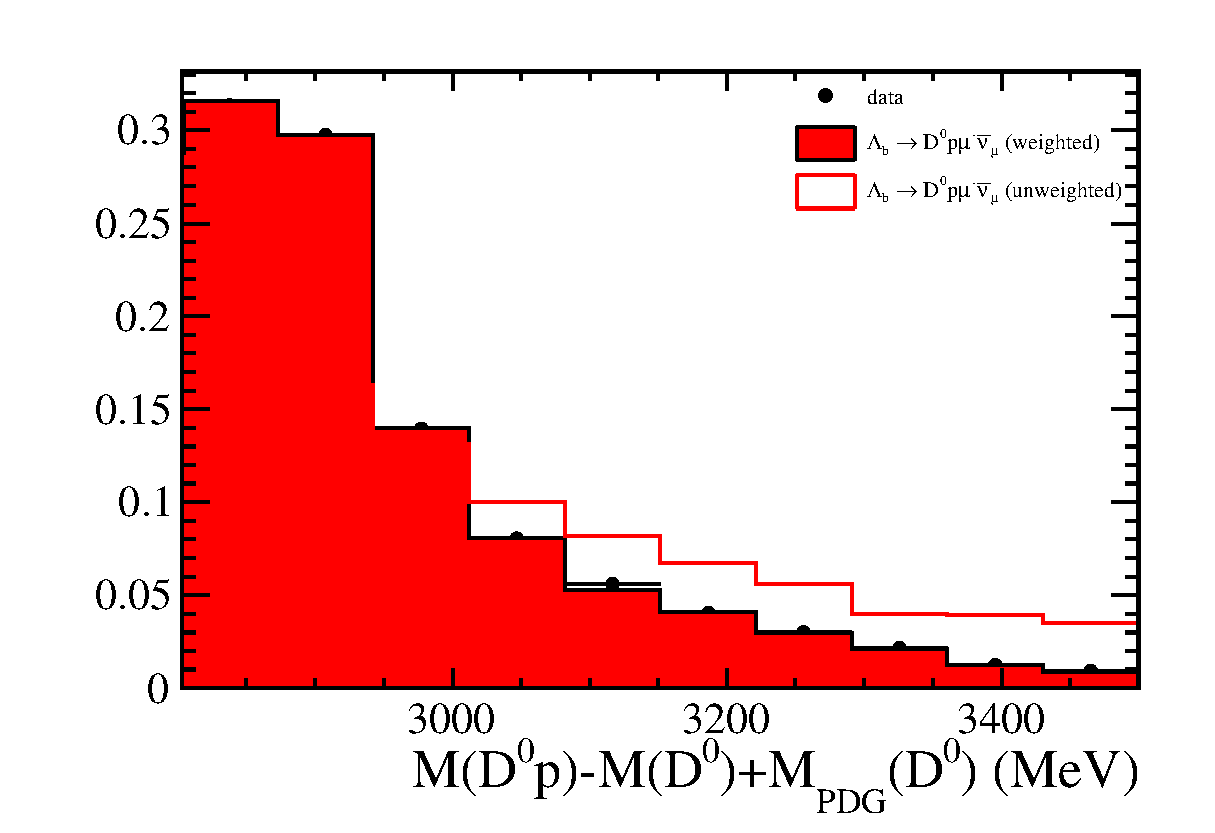
\includegraphics[width=0.32\textwidth]{LbToD0p/comparisons/3D/mD0p_mD0mu_mD0pmu/20Bins/20.0MaxWeight/Bh_DELTA_MASS}
	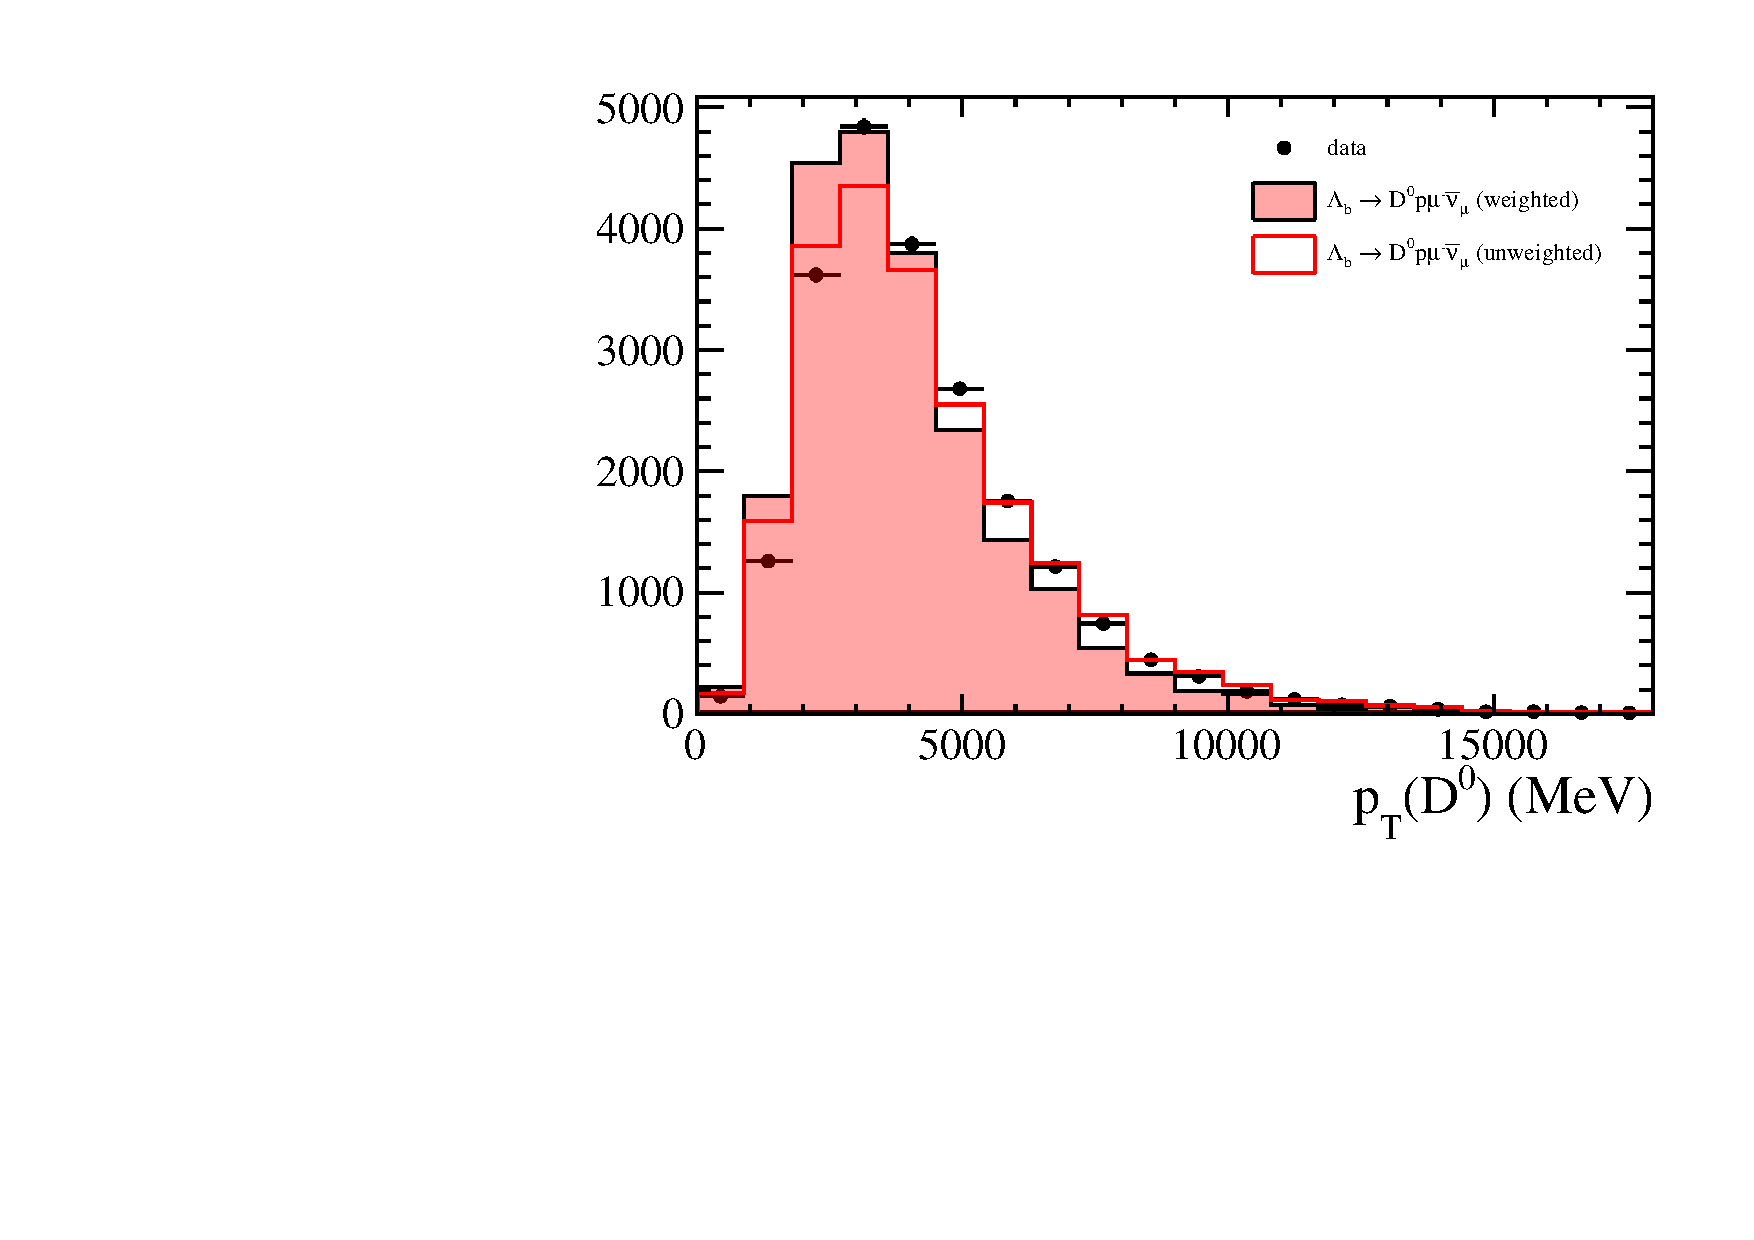
\includegraphics[width=0.32\textwidth]{LbToD0p/comparisons/3D/mD0p_mD0mu_mD0pmu/20Bins/20.0MaxWeight/D0_PT}
	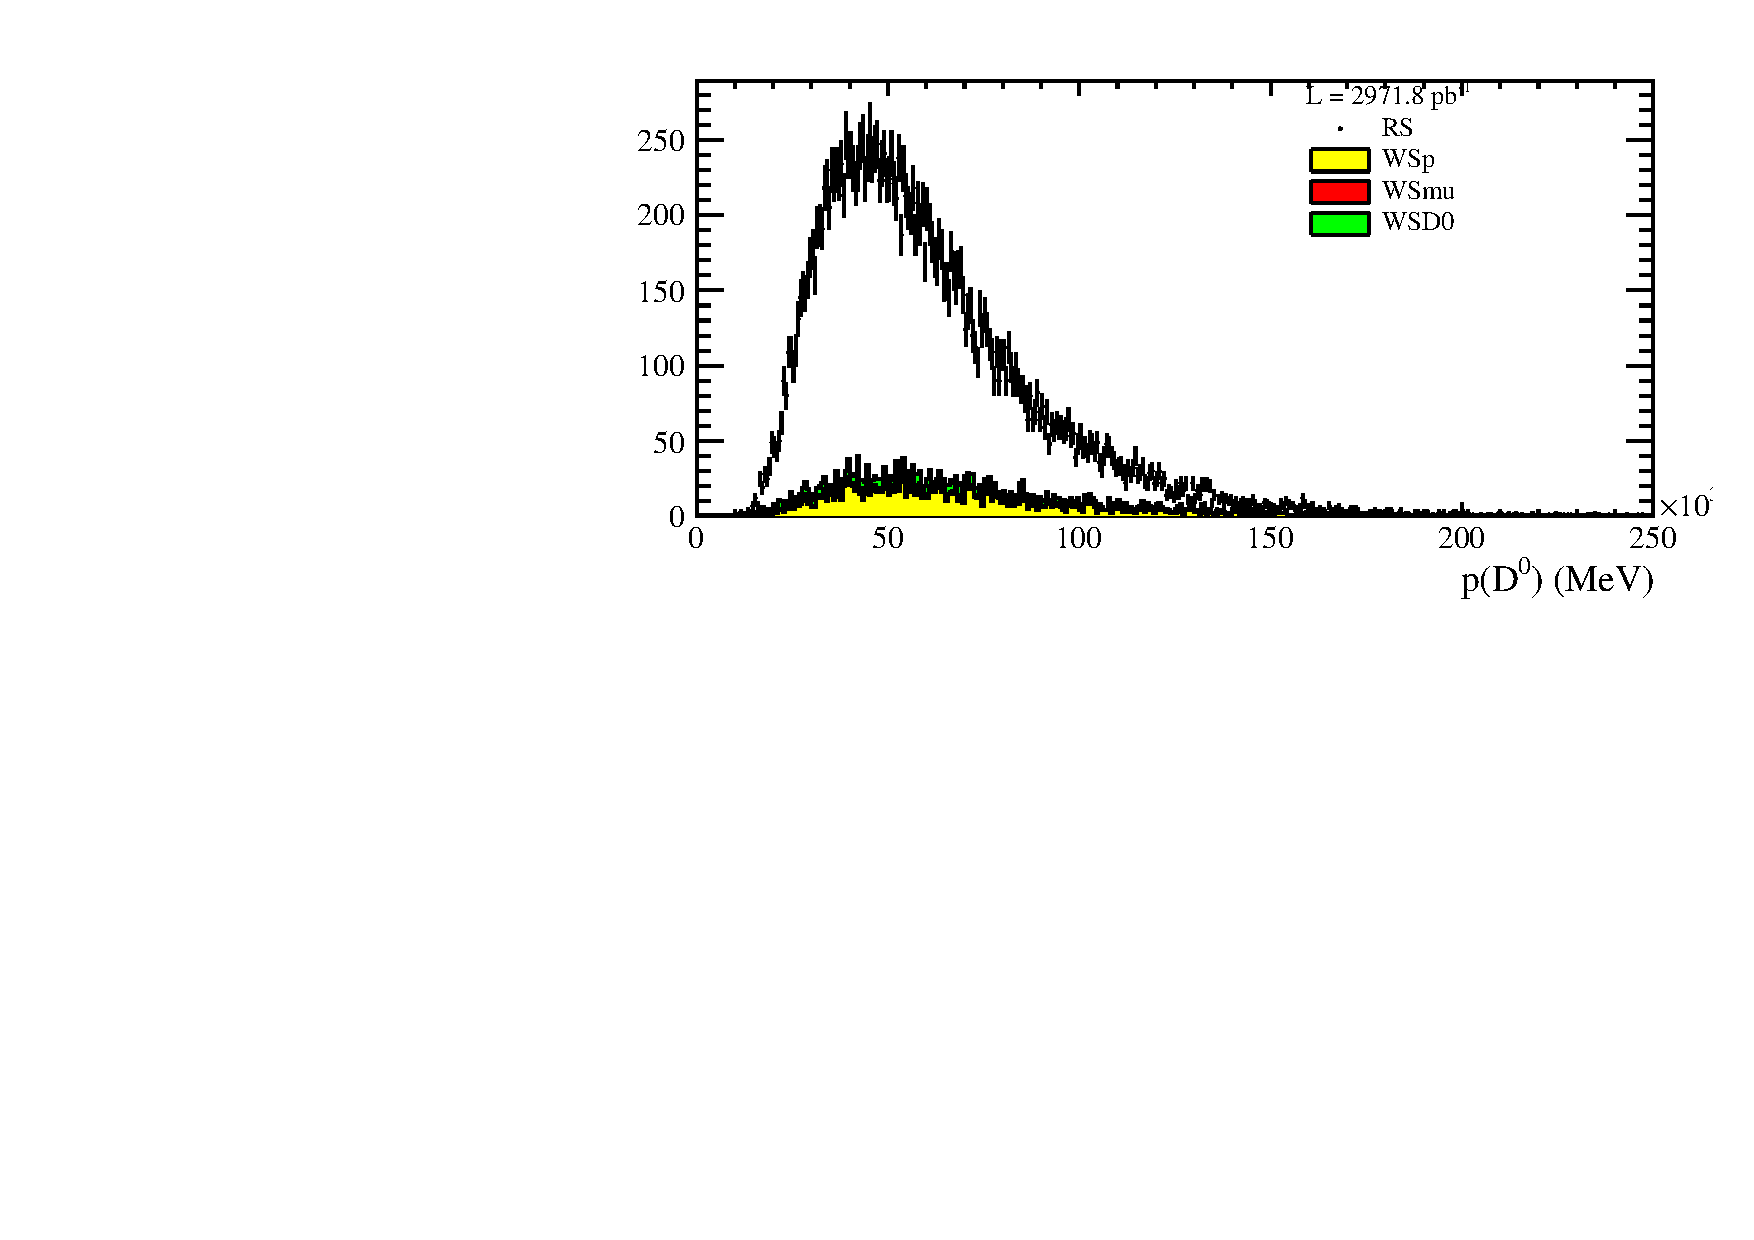
\includegraphics[width=0.32\textwidth]{LbToD0p/comparisons/3D/mD0p_mD0mu_mD0pmu/20Bins/20.0MaxWeight/D0_P}          \\
    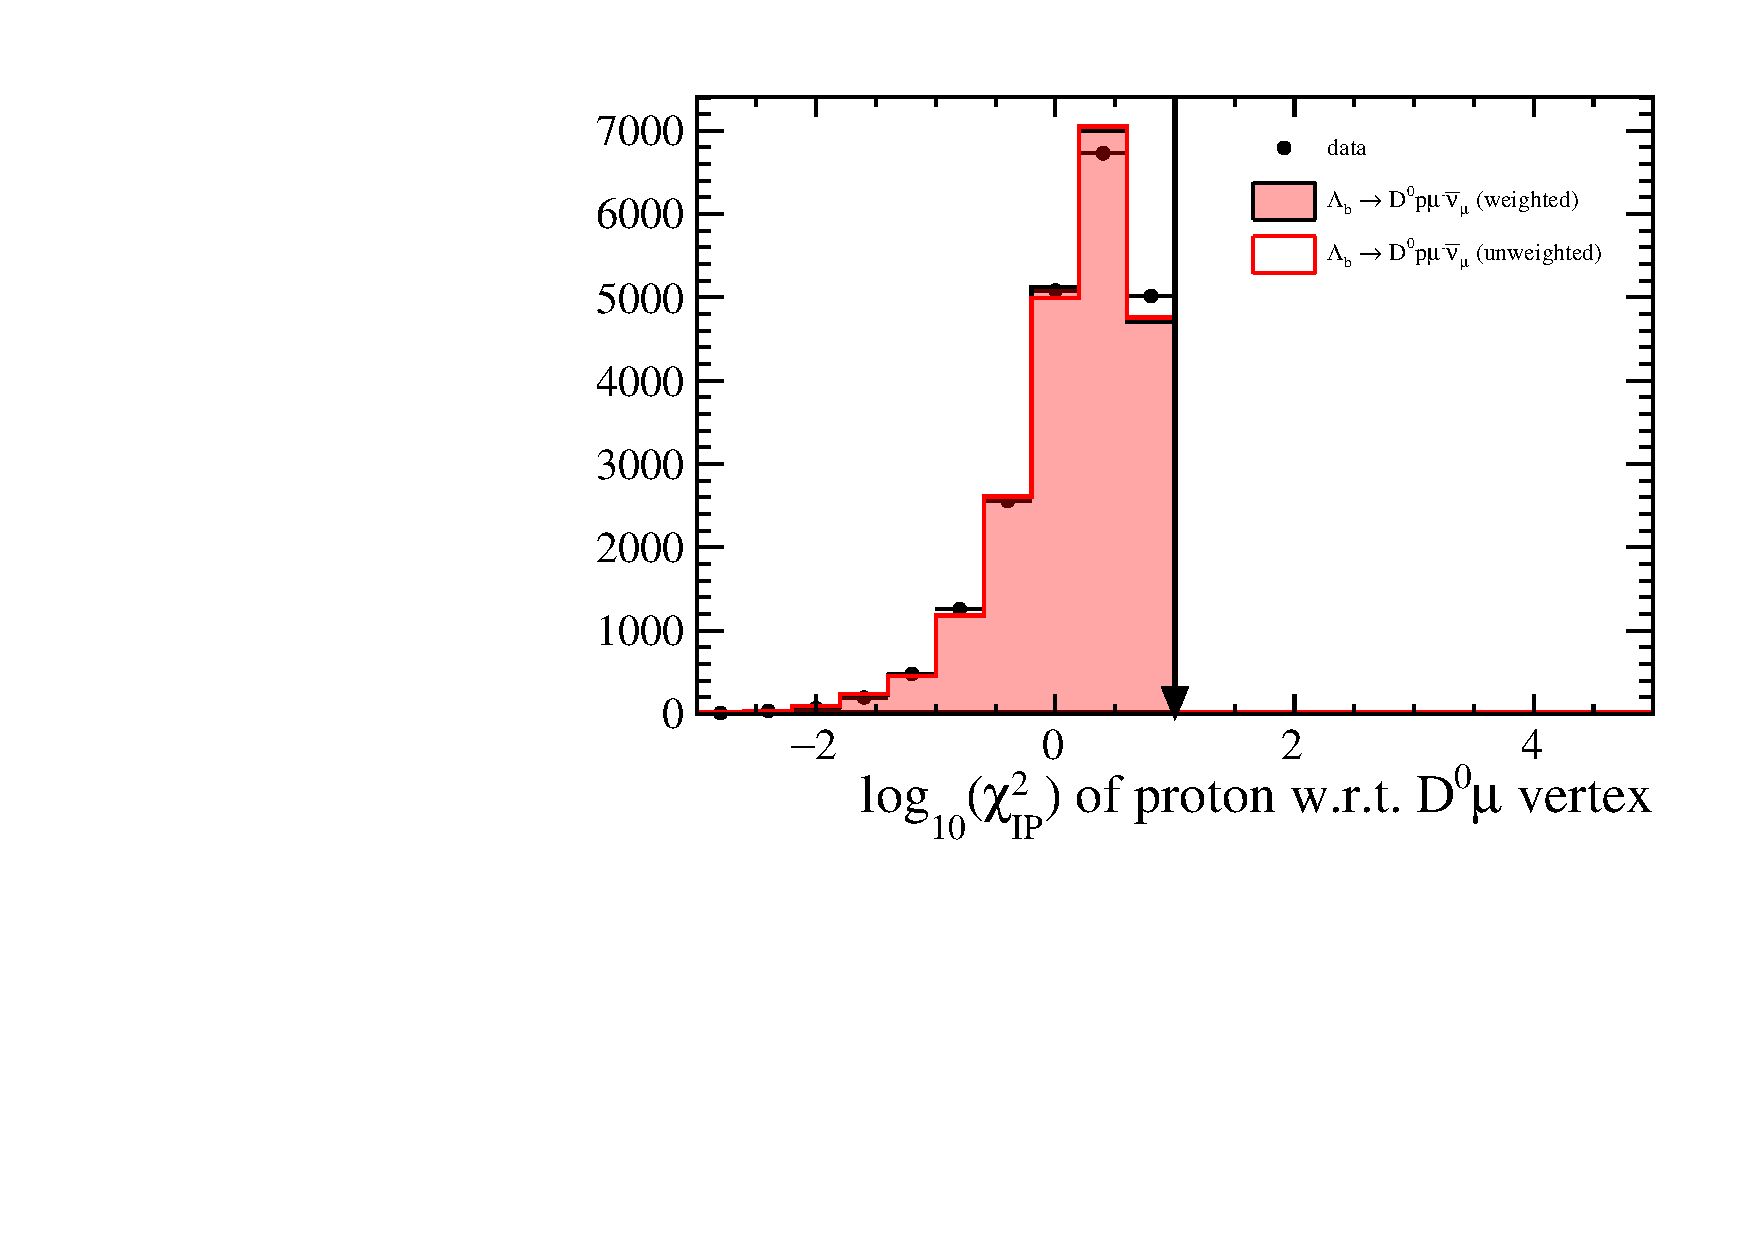
\includegraphics[width=0.32\textwidth]{LbToD0p/comparisons/3D/mD0p_mD0mu_mD0pmu/20Bins/20.0MaxWeight/logIP}
	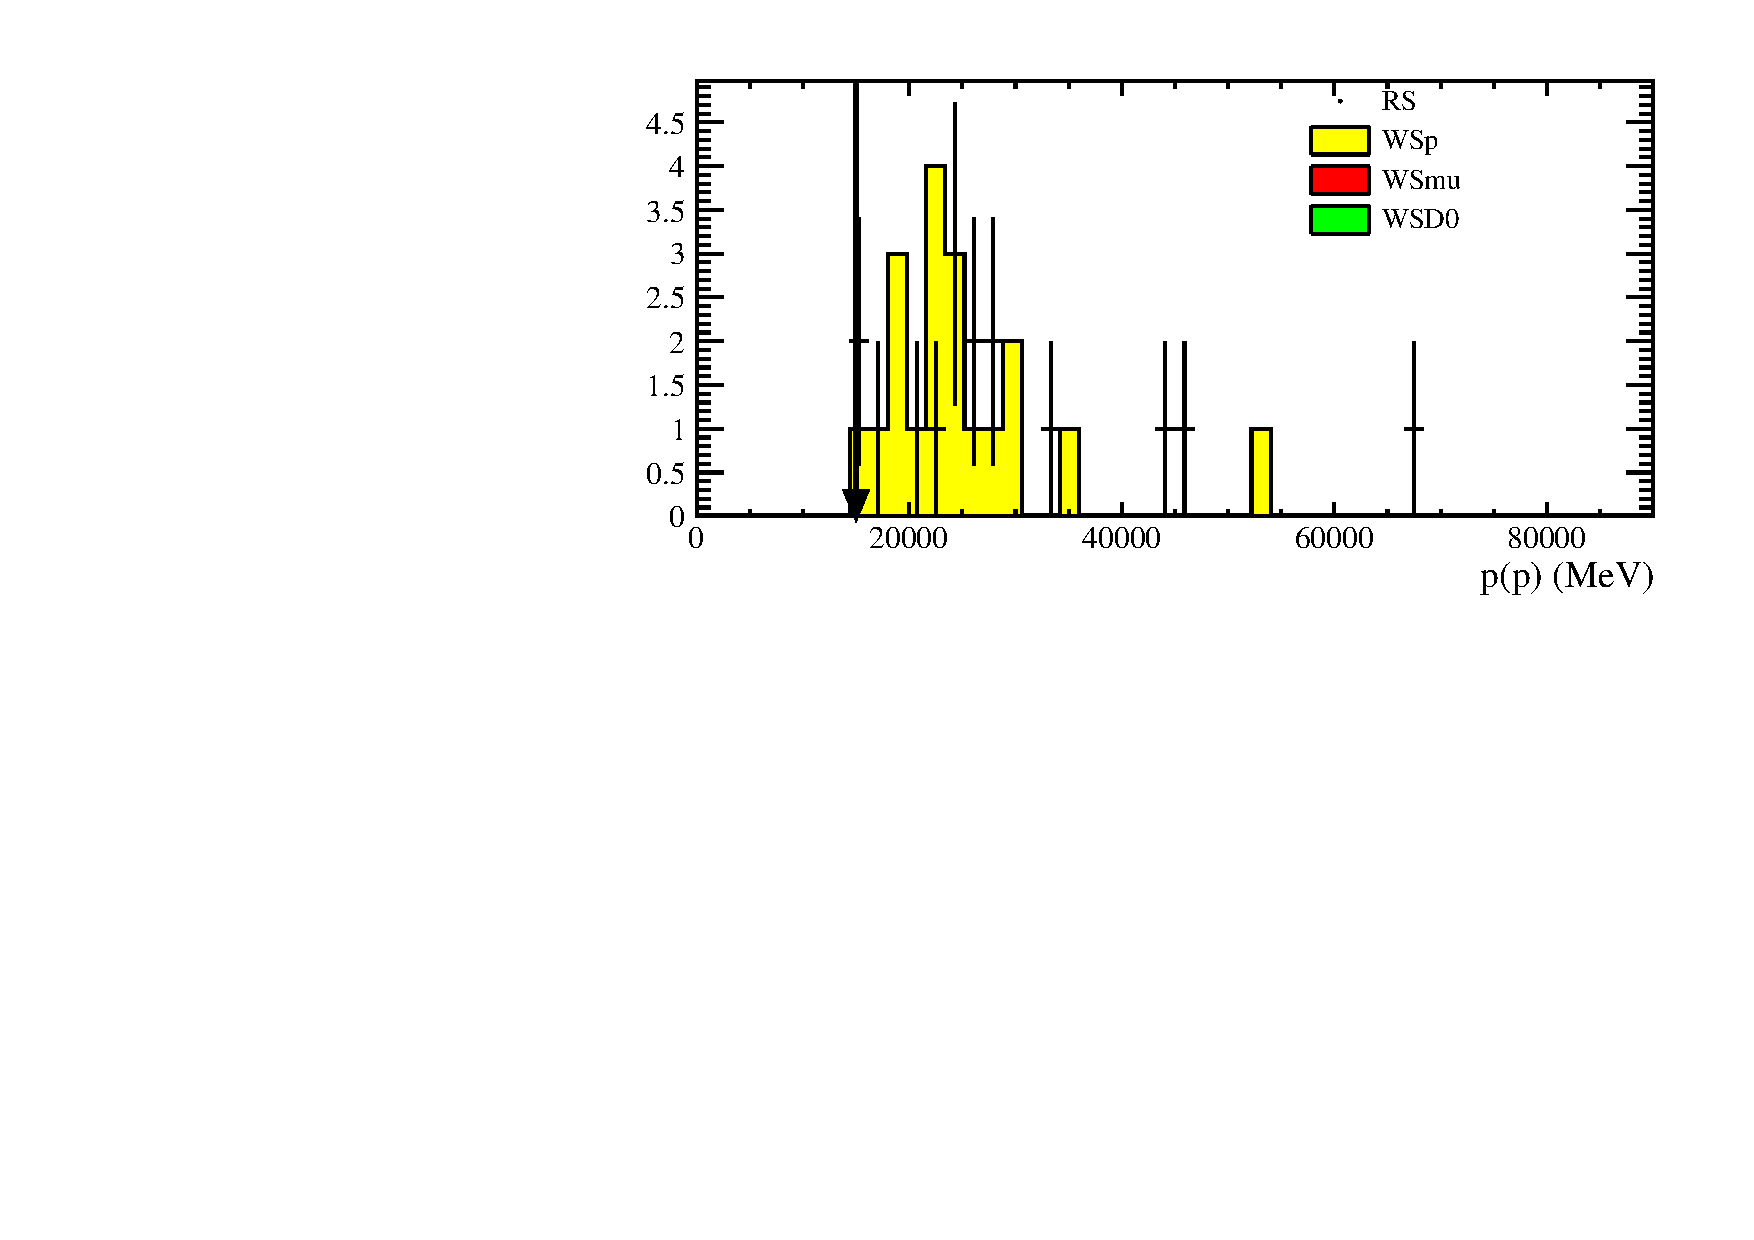
\includegraphics[width=0.32\textwidth]{LbToD0p/comparisons/3D/mD0p_mD0mu_mD0pmu/20Bins/20.0MaxWeight/h_P}
	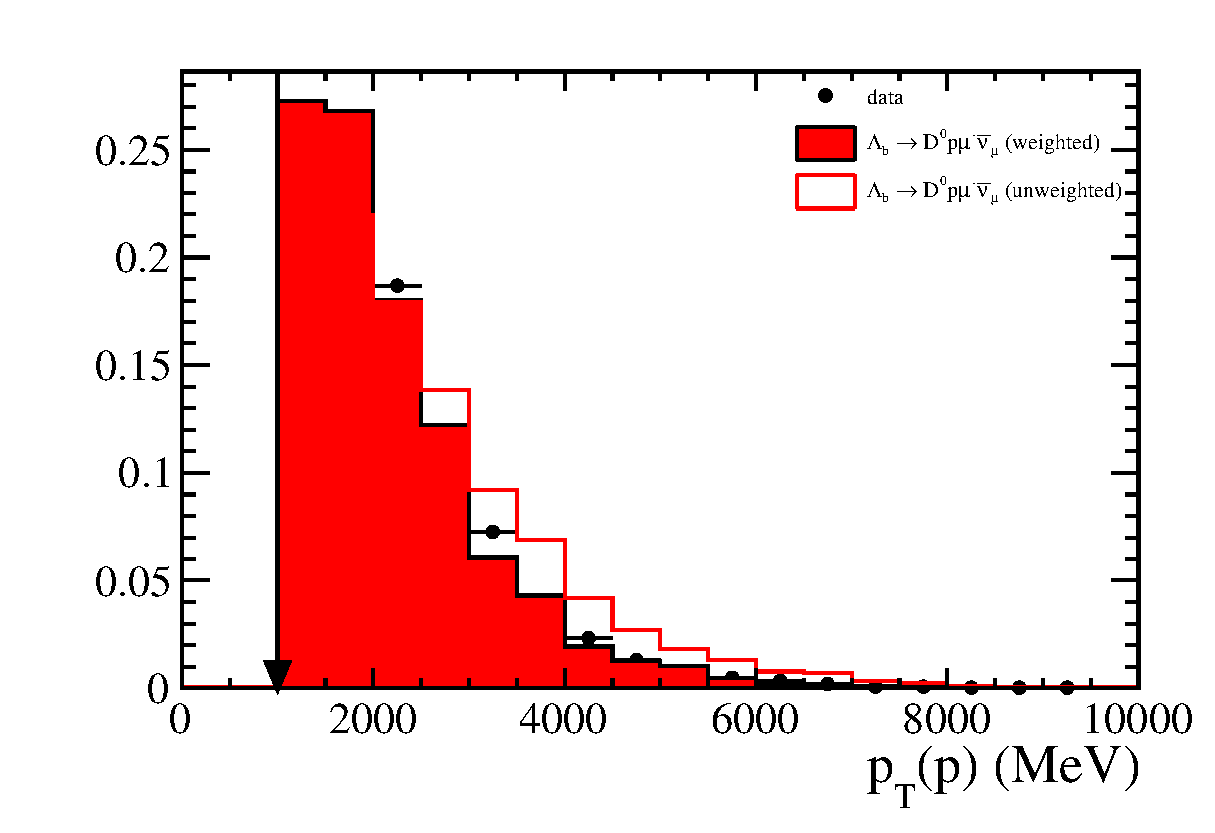
\includegraphics[width=0.32\textwidth]{LbToD0p/comparisons/3D/mD0p_mD0mu_mD0pmu/20Bins/20.0MaxWeight/h_PT}
	\caption{Comparison of data (black points) and simulation for the \LbToDpmunuX channel before (red line) and after (red shaded area) threedimensional reweighting as described in the text (see sec. \ref{sec:Reweight_D0p}).}
    \label{fig:reweight_D0p_app}
\end{figure}

\chapter{Reweighting and comparison of the \LbToLcmunu candidates}
\label{app:Reweight_Lc}
Except for the kinematic \pt(\Lb) reweighting no additional reweighting is applied as for \LbToDpmunu. 
However, the data is saturated by the decay \LbToLcmunu itself and decays into two excited states \decay{\Lb}{\LcstarRes{(2593)}\mun\neumb} and \decay{\Lb}{\LcstarRes{(2625)}\neumb}. 
Thus, figure \ref{fig:reweight_Lc_app} shows a comparison of sidebandsubtracted data and the sum of the three different channels.
They are summed up according to the yields obtained by the corrected mass fit (see section \ref{sec:Normalisationfit}).

\begin{figure}[tb]
	\centering
  	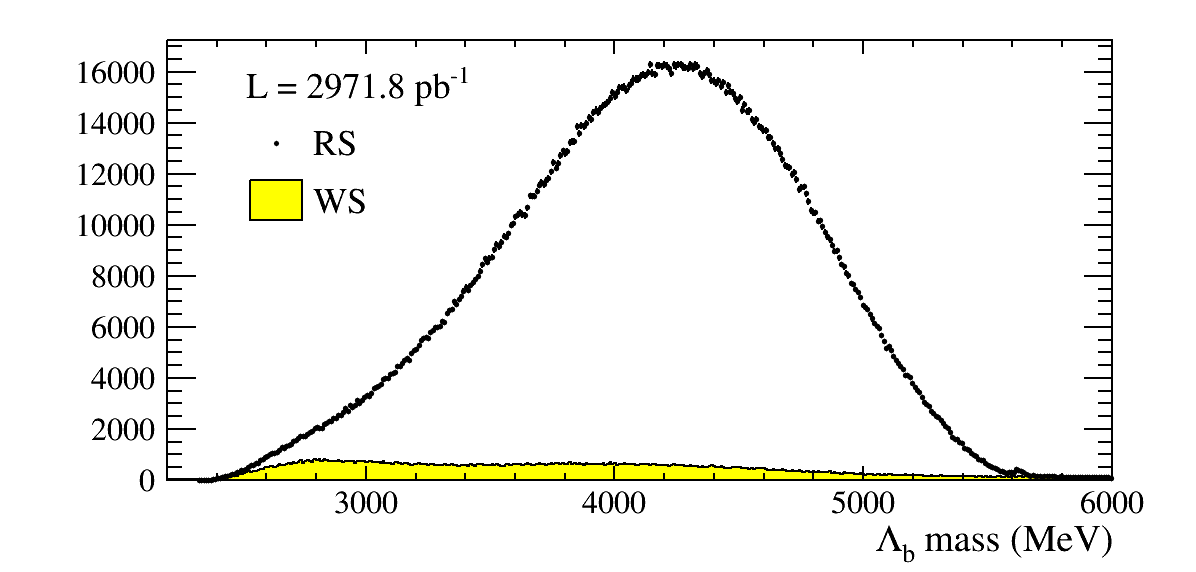
\includegraphics[width=0.49\textwidth]{LbToLc/comparisons/Lb_M}
  	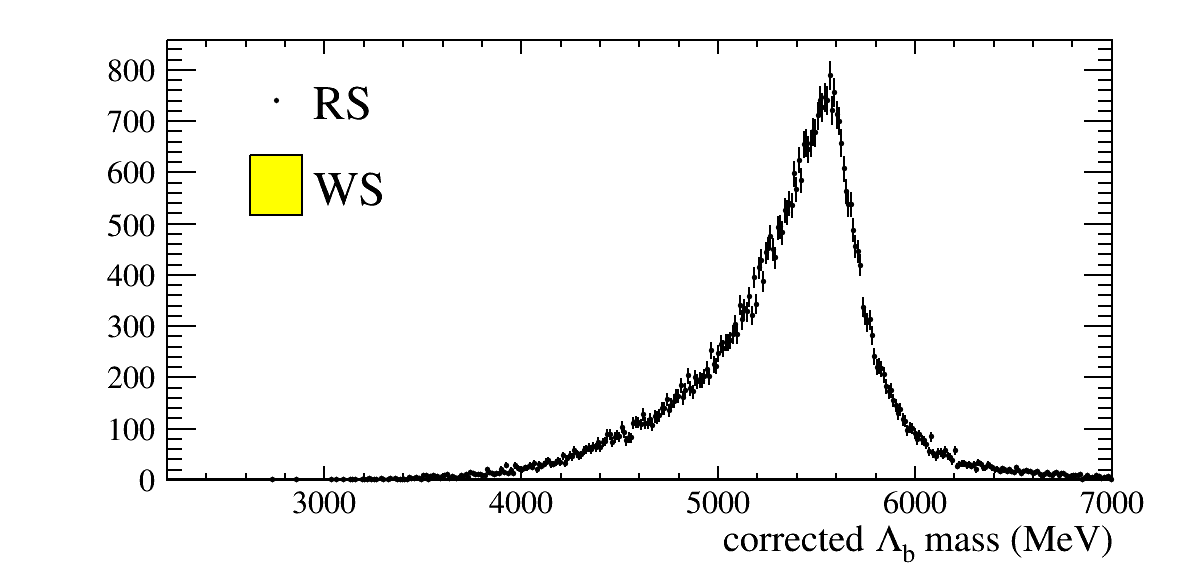
\includegraphics[width=0.49\textwidth]{LbToLc/comparisons/Lb_BPVCORRM}
  	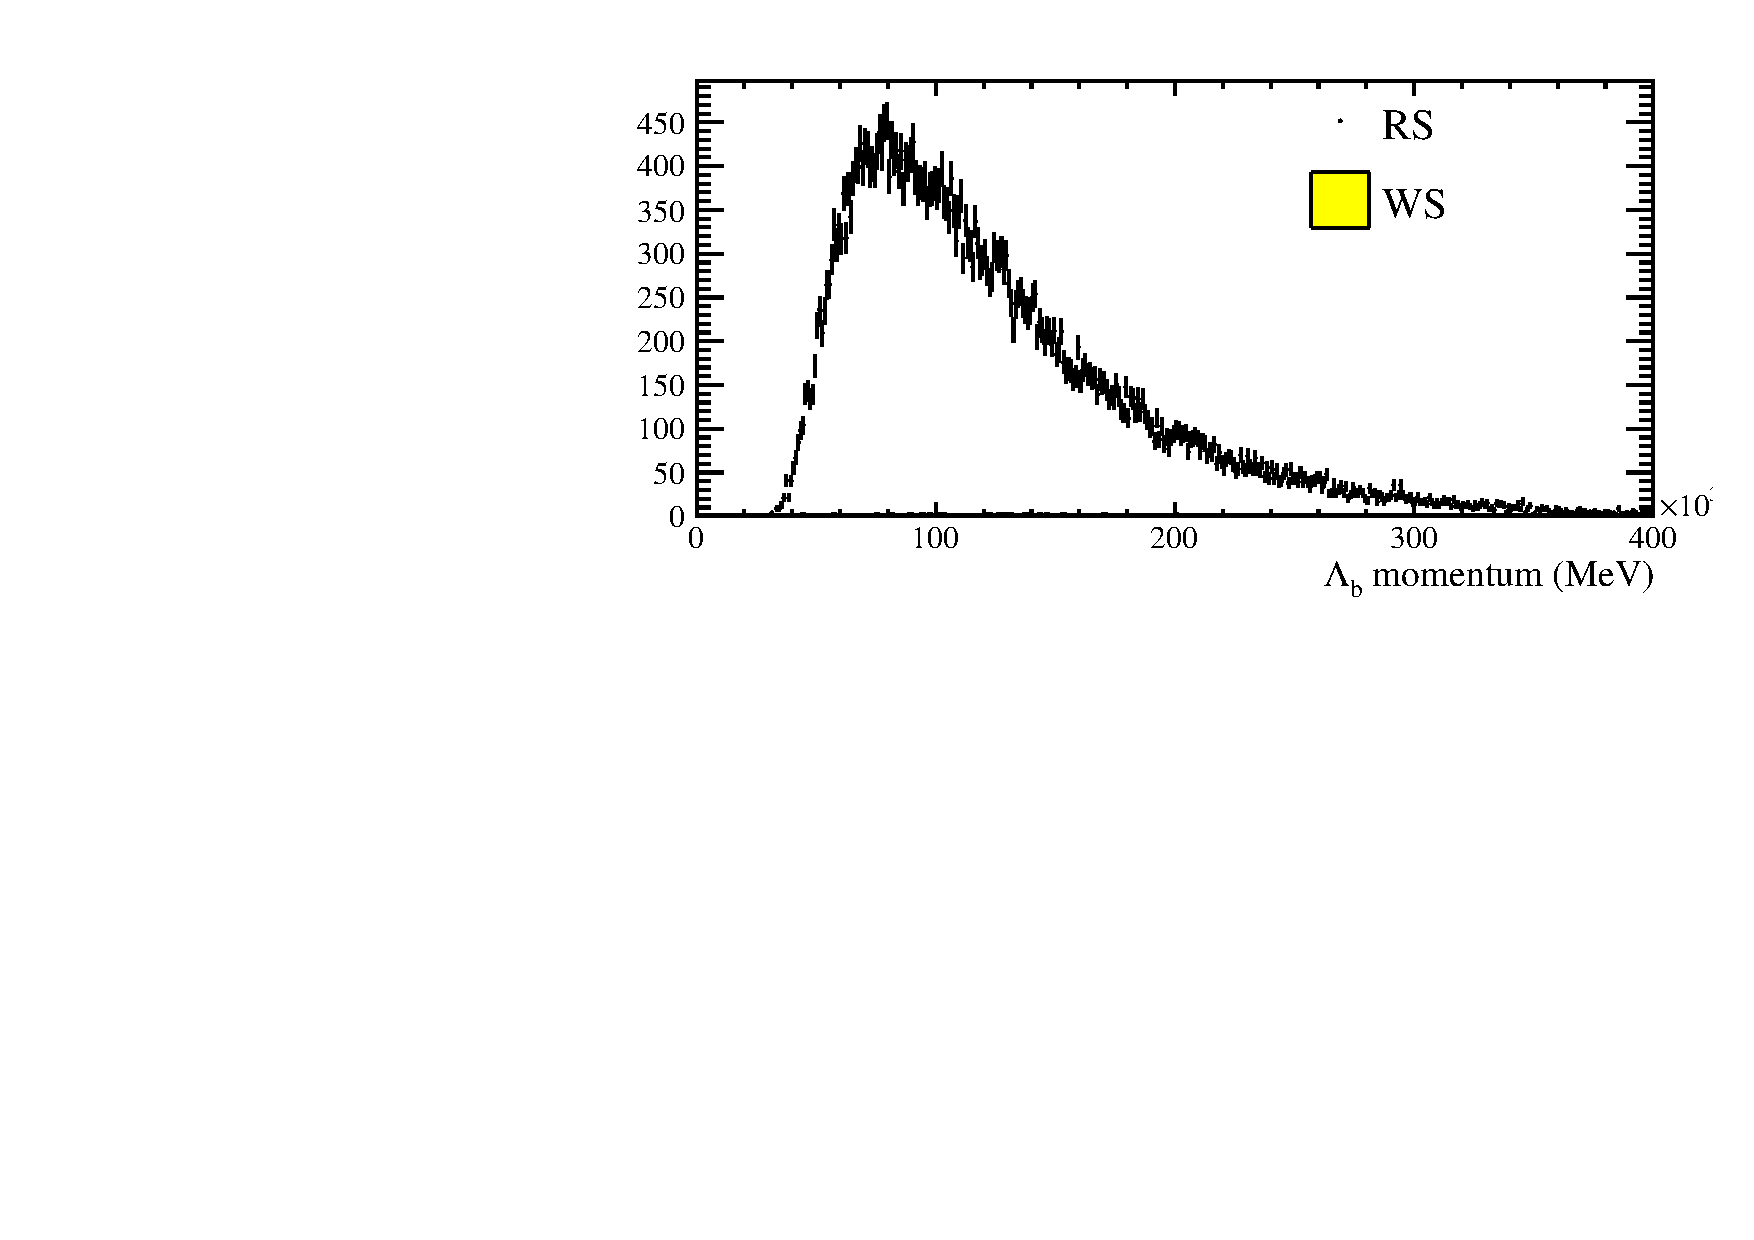
\includegraphics[width=0.49\textwidth]{LbToLc/comparisons/Lb_P}
  	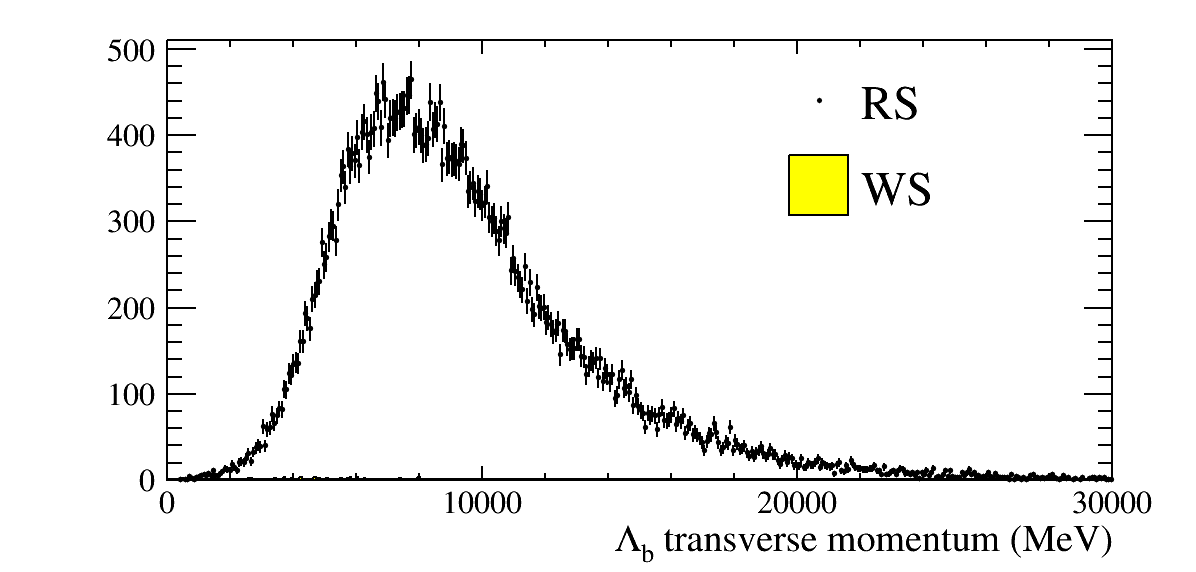
\includegraphics[width=0.49\textwidth]{LbToLc/comparisons/Lb_PT}
  	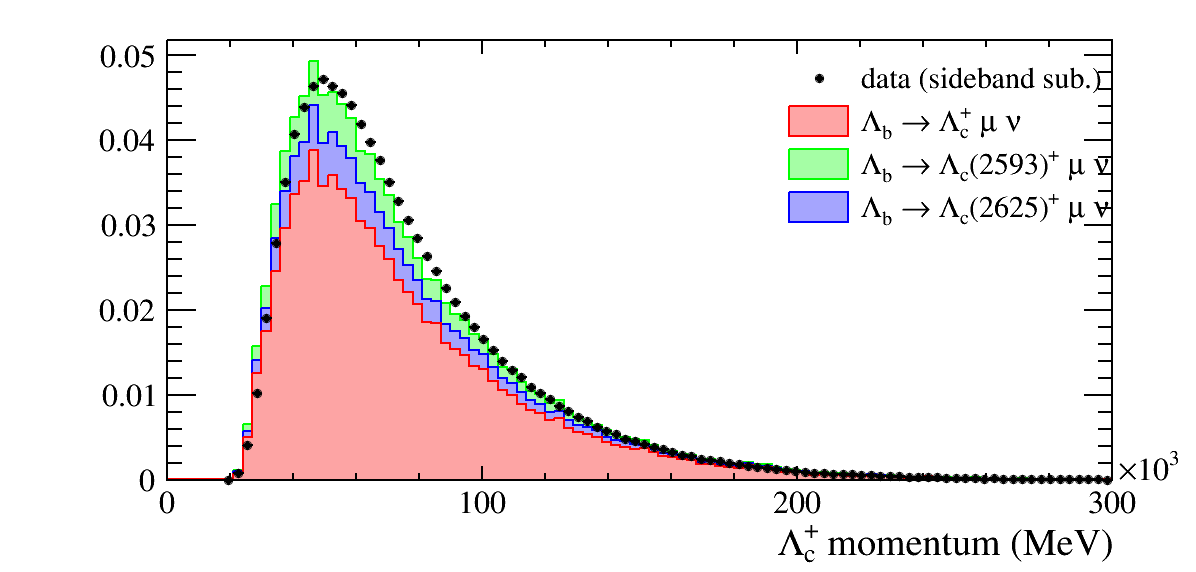
\includegraphics[width=0.49\textwidth]{LbToLc/comparisons/Lc_P}
  	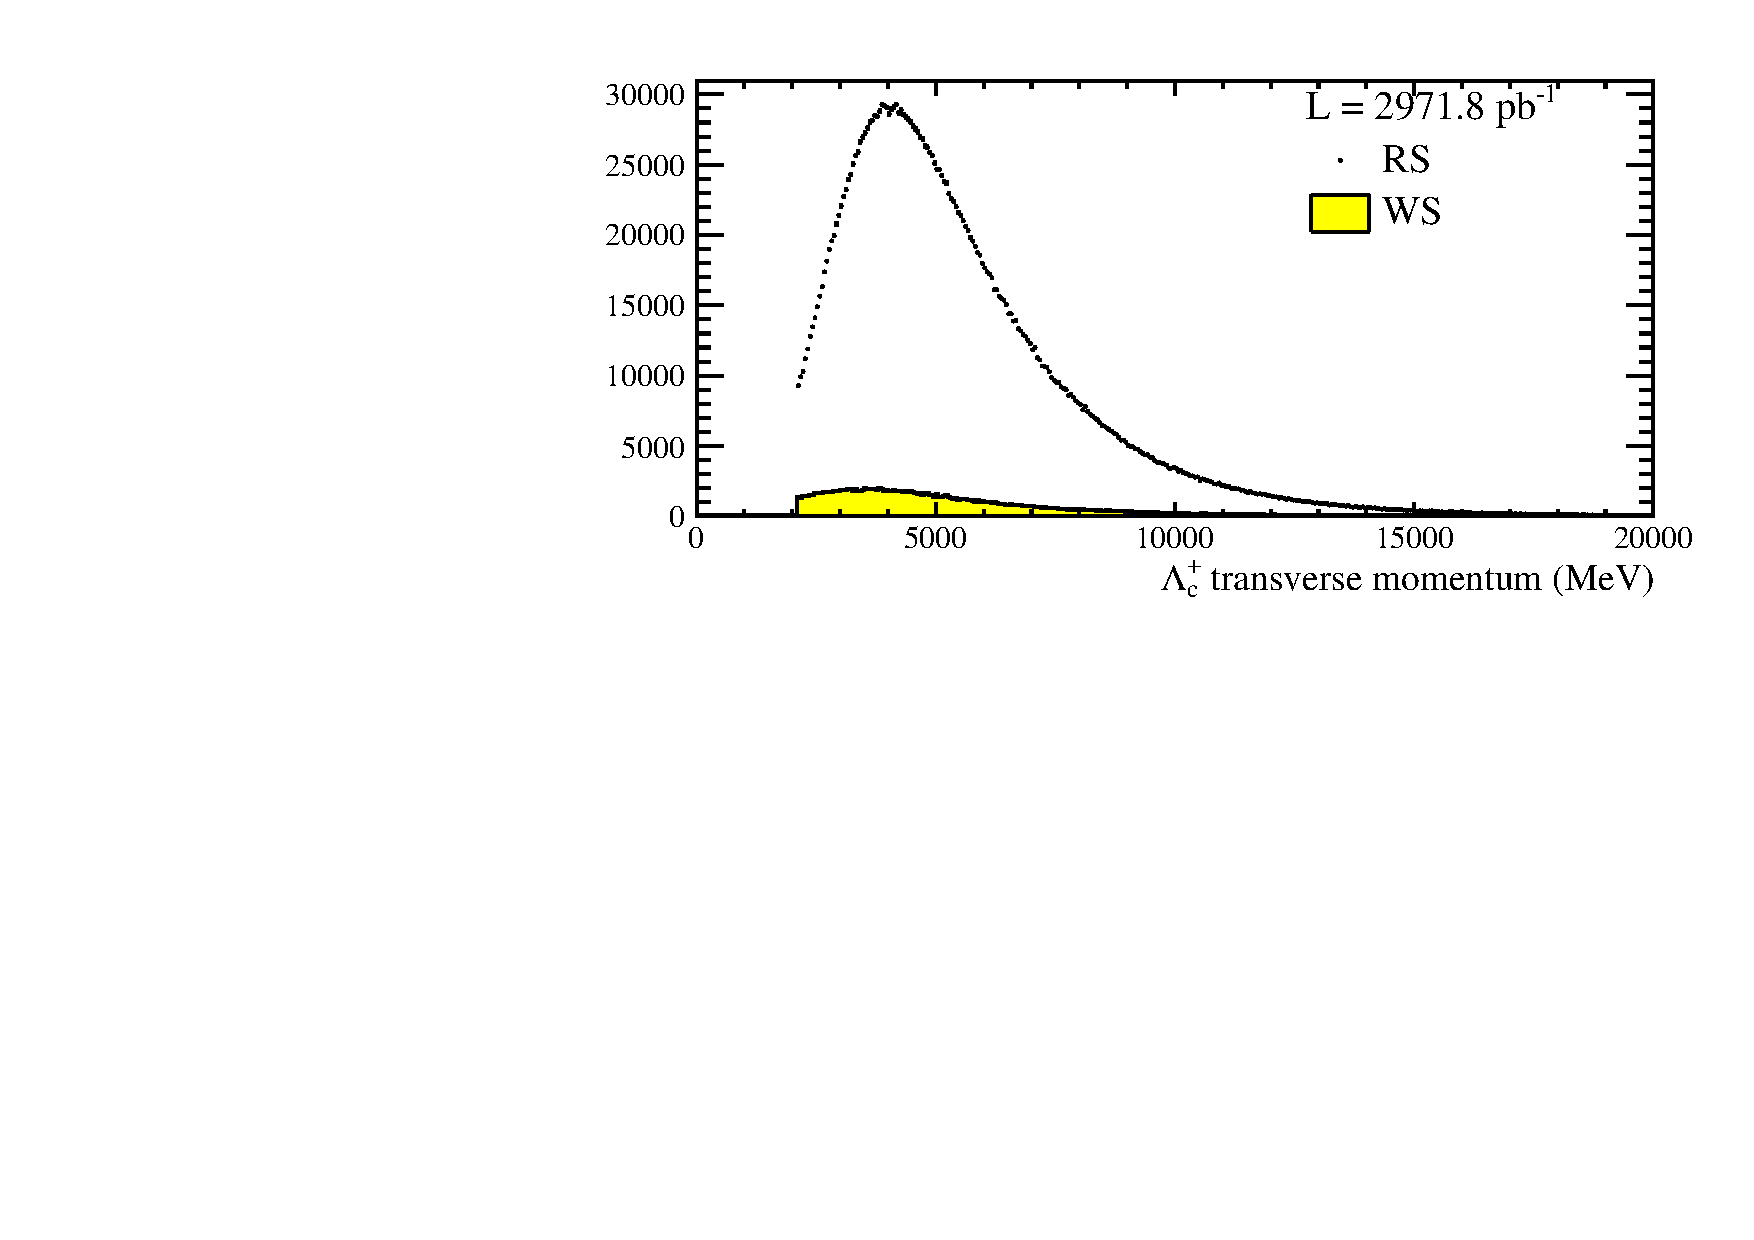
\includegraphics[width=0.49\textwidth]{LbToLc/comparisons/Lc_PT}
  	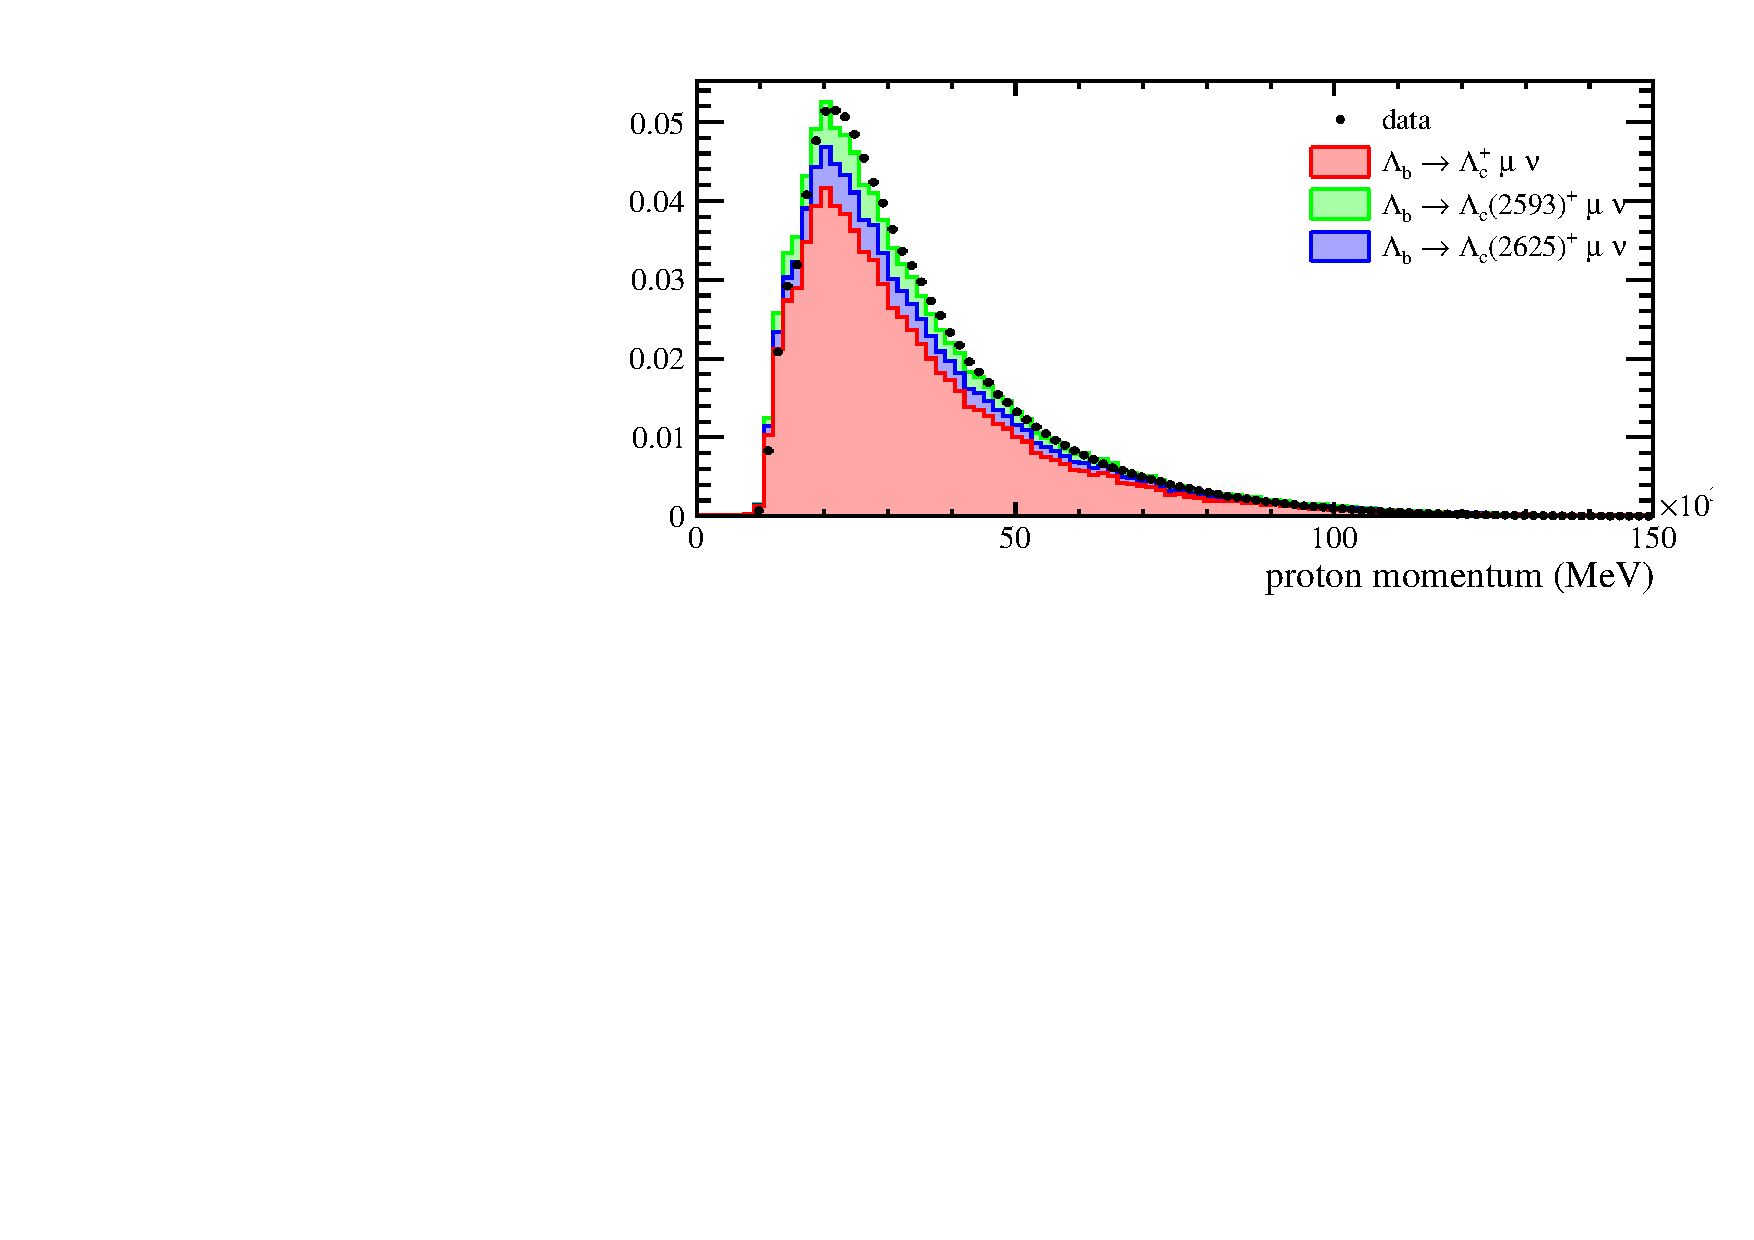
\includegraphics[width=0.49\textwidth]{LbToLc/comparisons/p_P}
  	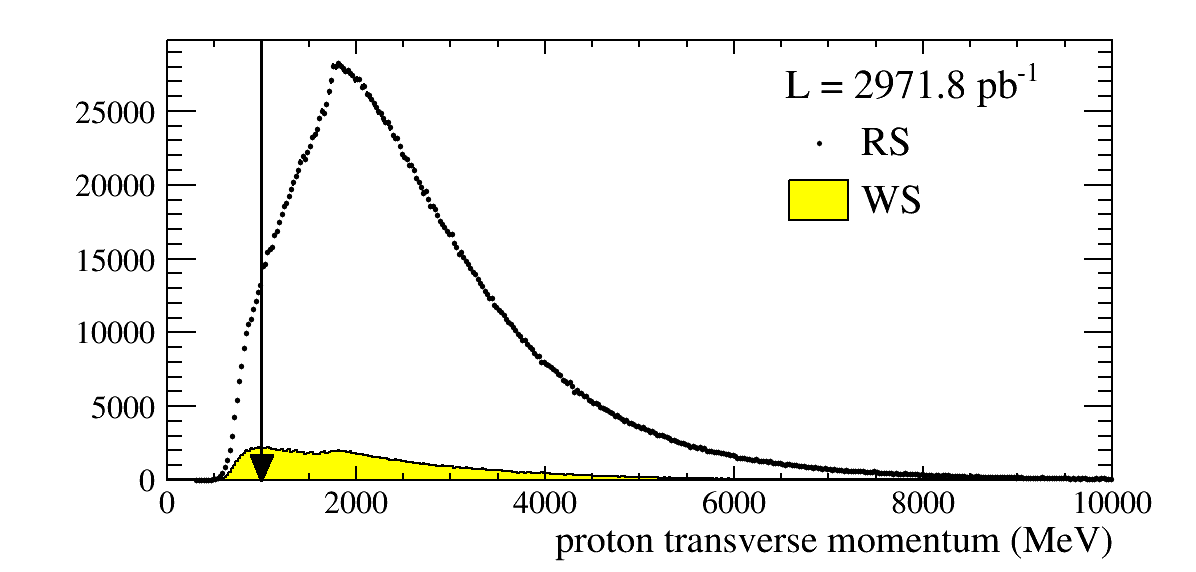
\includegraphics[width=0.49\textwidth]{LbToLc/comparisons/p_PT}
	\caption{Comparison of sidebandsubtracted data and the sum of the simulations describing the decays \LcTopKpi, \decay{\Lb}{\LcstarRes{(2593)}\mun\neumb} and \decay{\Lb}{\LcstarRes{(2625)}\mun\neumb}. Only the kinematic \pt(\Lb) reweighting is applied.}
    \label{fig:reweight_Lc_app}
\end{figure}

